\documentclass[twoside]{article}

\usepackage[preprint]{aistats2027}

\usepackage[round]{natbib}
\renewcommand{\bibname}{References}
\renewcommand{\bibsection}{\subsubsection*{\bibname}}

\usepackage[utf8]{inputenc}
\usepackage[hypertexnames=false,colorlinks=true,linkcolor=blue!55!black,citecolor=blue!55!black,urlcolor=blue!55!black]{hyperref}
\usepackage{url}
\usepackage{booktabs}
\usepackage{amsmath}
\usepackage{amssymb}
\usepackage{amsthm}
\usepackage{amsfonts}
\usepackage{nicefrac}
\usepackage{microtype}
\usepackage{xcolor}
\usepackage{graphicx}
\usepackage{array}
\usepackage{multirow}
\usepackage{algorithm}
\usepackage{algorithmic}
\usepackage[capitalize,noabbrev]{cleveref}

\newtheorem{proposition}{Proposition}

\newcommand{\sd}[1]{\,{\scriptsize$\pm$\,#1}}
\hyphenation{naPINN OrPINN PINN-EBM LAD-PINN MAD-PINN}
\newcommand{\pmstd}[2]{#1\,\text{\scriptsize($#2$)}}
\newcommand{\rej}{\lambda_{\mathrm{rej}}}
\newcommand{\sigrun}{\sigma_{\mathrm{run}}}
\newcommand{\wpde}{w_{\mathrm{PDE}}}
\newcommand{\sg}{\operatorname{sg}}
\DeclareMathOperator{\sig}{sig}
\DeclareMathOperator{\softplus}{softplus}
\renewcommand{\labelitemi}{$\bullet$}

\setlength{\emergencystretch}{1.5em}

\hypersetup{pdftitle={naPINN: Noise-Adaptive Physics-Informed Neural Networks for Recovering Physics from Corrupted Measurements},pdfauthor={Hankyeol Kim, Pilsung Kang}}

\begin{document}

\runningtitle{naPINN: Noise-Adaptive Physics-Informed Neural Networks}
\runningauthor{Hankyeol Kim, Pilsung Kang}

\twocolumn[

\aistatstitle{naPINN: Noise-Adaptive Physics-Informed Neural Networks \\
for Recovering Physics from Corrupted Measurements}

\aistatsauthor{
Hankyeol Kim \qquad
Pilsung Kang$^{\dagger}$\\[4pt]
{\normalsize
Department of Industrial Engineering, Seoul National University}\\
{\normalsize Seoul, Republic of Korea}\\[2pt]
{\small\ttfamily
\char`\{hankyeol, pilsung\_kang\char`\}@snu.ac.kr}\\[4pt]
{\footnotesize
\qquad
$^{\dagger}$Corresponding author.}
}

\aistatsaddress{} ]

\begin{abstract}
Inverse physics-informed neural networks (PINNs) recover fields and PDE coefficients from sparse measurements, but they are vulnerable to corrupted data, and even a few faulty sensors can bias the recovered physics. Real measurement noise is rarely Gaussian and its form is unknown in advance, so no single fixed loss suits every case. We present \textbf{naPINN}, a noise-adaptive PINN that learns during training how much to trust each measurement and weights the data accordingly. It learns the residual distribution online, converts it into a per-measurement weight through a trainable gate, and discourages discarding measurements with a rejection cost. On three simulated benchmarks with multimodal noise and gross outliers, naPINN roughly halves the field error of the best fixed robust loss at the higher corruption levels and also improves on directly optimizing a learned noise likelihood. On real particle image velocimetry under a nominal Navier-Stokes model, it has the lowest field error of all methods tested and excludes about $99\%$ of corrupted components while keeping over $95\%$ of clean ones. An ablation shows that both the learned residual distribution and the adaptive gate are necessary.
\end{abstract}

% ====================================================================
\section{INTRODUCTION}
\label{sec:intro}

Physics-informed neural networks (PINNs) combine observational data with
physical laws by training a neural network to fit measurements while satisfying
a governing partial differential equation (PDE)
\citep{Raissi2019, Karniadakis2021}. This makes them a natural tool for inverse
problems, in which a full field and unknown physical coefficients must be
recovered from sparse measurements, such as inferring velocity and pressure from
flow visualizations \citep{Raissi2020} or estimating subsurface flow parameters
\citep{Tartakovsky2020}. Real measurements, however, are often corrupted by
sensors that drift, saturate or fail, and may contain gross outliers. Standard
PINNs fit the data with a mean squared error, which implicitly assumes Gaussian
noise and gives the largest residuals the largest gradients. Even a few faulty
sensors can then bias both the reconstructed field and the recovered
coefficients. Such corruption is common in experimental and field data, yet most
work on PINNs assumes clean or Gaussian-noise measurements and concentrates on
improving optimization \citep{Wang2021, McClenny2023}.

Existing robust PINNs fix how they treat corruption before training. Robust
losses such as $\ell_1$ fitting \citep{Peng2022} or a $q$-Gaussian likelihood
\citep{Duarte2025} assume a noise family, and residual screening
\citep{Peng2022} requires a threshold chosen before the noise is known. Neither
choice can be made reliably when the noise is asymmetric or multimodal.
PINN-EBM \citep{Pilar2024} removes the need for a fixed noise family by learning
the noise density from the residuals and using its negative log-likelihood as
the data loss. However, it is designed for homogeneous noise and does not assess
the reliability of individual measurements.

Our key observation is that a learned noise density is most useful for deciding
which measurements to trust, not as the training objective. A density estimated
during training is imperfect, but it can still tell typical residuals from
atypical ones. Building on this idea, we propose the Noise-Adaptive PINN
(\textbf{naPINN}) (\cref{fig:framework}). naPINN learns the distribution of
measurement residuals during training and treats measurements whose residuals
are unlikely under this distribution as less reliable. A trainable gate
converts this likelihood into a reliability weight for each measurement and
learns how unlikely a residual must be before the measurement is excluded,
while a rejection cost discourages it from discarding valid data. Because
reliability is judged by likelihood and not by residual magnitude, a large
residual that lies on a mode of asymmetric or multimodal noise is kept, whereas
an isolated gross outlier is excluded.
naPINN changes only how measurements are weighted, so it can be added to an
existing PINN without modifying its network or data loss, and it improves every
backbone architecture we tested.

We evaluate naPINN on three simulated benchmarks and on real particle image
velocimetry (PIV) from RealPDEBench \citep{hu2026realpdebench}, where the
Navier--Stokes residual only approximates the measured flow. With a plain
squared loss, naPINN reduces the field error of the best robust loss by a factor
of $2.0$ to $2.4$ at $15\%$ gross outliers and is more accurate than PINN-EBM in
seven of nine simulated settings. On real PIV its error is $31\%$ lower than
that of the best baseline at $15\%$ injected corruption, and its gate excludes
about $99\%$ of the corrupted components while keeping over $95\%$ of the
others. An ablation shows that neither the learned residual density nor the trainable
gate suffices on its own.

Our contributions are as follows.
\begin{itemize}
\setlength{\itemsep}{0pt}
\item We propose naPINN, which learns the distribution of measurement
residuals during training and assigns each measurement a reliability weight
through a trainable gate, with a rejection cost that discourages discarding
valid data.
\item We show that the naPINN objective relaxes a trimmed squared loss in which
measurements are selected by the learned density, and characterize where the
learned cutoff settles.
\item We compare naPINN with robust-loss, Bayesian, learned-likelihood and
screening baselines on simulated benchmarks and on real PIV under a nominal PDE,
and isolate the roles of the learned density and the trainable gate by
ablation.
\end{itemize}

\begin{figure*}[t]
\centering
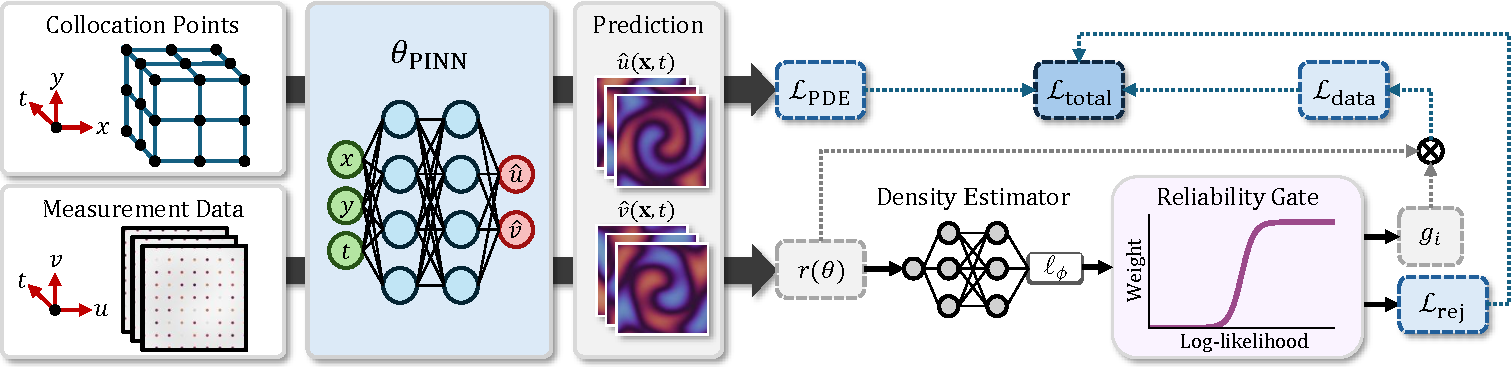
\includegraphics[width=0.95\textwidth]{figures/framework.pdf}
\caption{The naPINN framework. The PINN $\hat u_\theta$ is trained on a PDE
loss and a gated data loss. A density estimator with parameters $\phi$ (here an
EBM) scores the normalized residuals, a reliability gate maps the standardized
log-density to a weight $g_i$ on the data loss, and the rejection cost
$\mathcal{L}_{\mathrm{rej}}$ penalizes exclusion.}
\label{fig:framework}
\end{figure*}

% ====================================================================
\section{RELATED WORK}
\label{sec:related}

\paragraph{Stabilizing PINN training.}
A large body of work addresses optimization difficulties in PINNs, such as
spectral bias, stiffness and imbalanced gradients between loss terms
\citep{Rahaman2019, Wang2021, SWang2022, CWang2022}. Proposed remedies include
adaptive and gradient-based loss balancing
\citep{Chen2018, Xiang2022, Hwang2024, Bischof2025}, self-adaptive weights on
the residual and data terms \citep{McClenny2023}, adaptive sampling of
collocation points \citep{Nabian2021}, and region- or sample-level optimization
schemes \citep{Wu2024, Duan2025}. These methods weight loss terms, regions or
collocation points to improve optimization. They do not assess whether an
individual measurement is reliable.

\paragraph{Robust and probabilistic inverse PINNs.}
PINN variants for corrupted data change the data loss or screen the
measurements. \citet{Peng2022} use an $\ell_1$
(least-absolute-deviation) loss followed by median-based screening, which we
call LAD-PINN and MAD-PINN, and OrPINN \citep{Duarte2025} uses a $q$-Gaussian
likelihood. Both fix the noise model in advance. PINN-EBM \citep{Pilar2024}, the
closest method to ours, learns the noise density with a one-dimensional EBM
\citep{LeCun2006} and uses its negative log-likelihood as the data loss.
naPINN uses the same kind of learned density, but to set a reliability weight
for each measurement instead of as the data loss. Bayesian PINNs (B-PINNs) \citep{Yang2021} and other probabilistic PINNs
\citep{Yang2019} quantify uncertainty under an assumed likelihood and are
complementary to measurement weighting.

\paragraph{Reliability-aware learning.}
Learning from corrupted supervision often selects or reweights samples by
confidence or small-loss criteria \citep{Natarajan2013, Jiang2018, Han2018, Li2020},
including self-paced learning \citep{Kumar2010}. Robust statistics bounds or trims the influence of large residuals
\citep{Huber1973, Hampel1974, Rousseeuw1984}. Anomaly detection scores sample
reliability with one-class objectives, reconstruction errors or density
estimates \citep{Chandola2013, Ruff2018, Pang2021}, and test-time adaptation
selects reliable samples before updating a model \citep{Yang2024, Wang2024DSS},
since model performance degrades under corrupted or shifted inputs
\citep{Hendrycks2019, Ovadia2019}. naPINN brings this reliability-aware view to
inverse PDE problems with a learned residual density and a trainable gate.

% ====================================================================
\section{METHOD}
\label{sec:method}

\subsection{Problem Setting}
Consider a PDE $\mathcal{N}[u](\mathbf{x},t;\boldsymbol{\eta}) = f(\mathbf{x},t)$
on a domain $\Omega \times [0,T]$ with an unknown coefficient $\boldsymbol{\eta}$.
We observe sparse measurements
\begin{equation}
y_i = u(\mathbf{x}_i, t_i) + \epsilon_i, \qquad i = 1,\dots,N_d,
\label{eq:measure}
\end{equation}
where the noise $\epsilon_i$ has an unknown distribution that may include gross
outliers. A network $\hat u_\theta$ approximates $u$. A PINN is generally trained
on a weighted sum of PDE, boundary, initial and data losses. We consider the realistic
measurement-driven setting in which boundary and initial conditions are not
available, so only the PDE and data terms remain. On $N_c$ collocation points
the PDE loss is
\begin{equation}
\mathcal{L}_{\mathrm{PDE}} = \frac{1}{N_c}\sum_{j=1}^{N_c}
\big\| \mathcal{N}[\hat u_\theta](\mathbf{x}_j,t_j;\boldsymbol{\eta})
- f(\mathbf{x}_j,t_j) \big\|^2 ,
\label{eq:pde}
\end{equation}
and the standard data loss is
$\mathcal{L}_{\mathrm{MSE}} = \frac{1}{N_d}\sum_i r_i^2$ with residual
$r_i = y_i - \hat u_\theta(\mathbf{x}_i, t_i)$. Robust-loss PINNs replace the
squared loss with another per-measurement loss $\rho(r_i)$, such as $\ell_1$ or a
$q$-Gaussian negative log-likelihood. For a field with several components, such
as the two velocity components in Burgers, each measured component is treated
as a separate measurement with its own residual and weight.

\subsection{Residual Density}
Residual magnitudes shrink as the PINN fits the data and vary from one
minibatch to another under gross outliers. Normalizing the residuals keeps the
input of the density estimator on a stable scale, but the statistics of a
single minibatch can be dominated by a few extreme residuals, especially early
in training. To stabilize both the estimator and the gate, we maintain a running
standard deviation $\sigrun \leftarrow (1-m)\,\sigrun + m\, s_{\mathcal{B}}$,
where $s_{\mathcal{B}}$ is the standard deviation of the minibatch residuals and
$m = 0.05$, and set $\tilde r_i = r_i/\sigrun$.

We model the distribution of the normalized residuals with a learned density
$p_\phi$, where $\phi$ denotes the parameters of the density estimator, and
write $\ell_\phi = \log p_\phi$. This density can be given by any estimator that
returns a log-density, such as a Gaussian mixture or a kernel density
estimate. We use a one-dimensional EBM by default, because it is a flexible
trainable density that requires no choice of component count or bandwidth.
The Gaussian mixture and the kernel density estimate give similar accuracy
(\cref{sec:practical,app:ablations}). The EBM defines
\begin{equation}
p_\phi(\tilde r) = \frac{\exp(-E_\phi(\tilde r))}{Z_\phi}, \qquad
Z_\phi = \int_{D} \exp(-E_\phi(s))\,ds,
\label{eq:ebm}
\end{equation}
where the energy $E_\phi$ is a small MLP and $Z_\phi$ is computed by trapezoidal
quadrature on the fixed interval $D = [-10, 10]$, so $p_\phi$ integrates to one
on $D$. Residuals outside $D$ are scored by the same network. Because
$\log Z_\phi$ is the same for every residual, it cancels when the gate
standardizes the log-densities below, so the gate weights depend only on the
energies $E_\phi(\tilde r_i)$ and not on how accurately $Z_\phi$ is computed.
The estimator is fitted by minimizing the finite-grid negative log-likelihood
\begin{equation}
\mathcal{L}_{\mathrm{est}}(\phi) = -\frac{1}{N_d}\sum_{i=1}^{N_d}
\ell_\phi\big(\sg(\tilde r_i)\big),
\label{eq:est}
\end{equation}
where $\sg$ is the stop-gradient operator, so fitting the estimator never
changes $\theta$.

\subsection{Reliability Gate and Objective}
Log-densities are standardized within each minibatch,
$z_i = \sg\big((\ell_\phi(\tilde r_i) - \mu_\ell)/\sigma_\ell\big)$, where
$\mu_\ell$ and $\sigma_\ell$ are the minibatch mean and standard deviation of
$\ell_\phi(\tilde r_i)$. A sigmoid gate maps $z_i$ to a reliability weight
\begin{equation}
g_i = \sig\!\big(a\,(z_i + \tau)\big),
\label{eq:gate}
\end{equation}
where the steepness $a = \softplus(\tilde a)$ and the cutoff
$\tau = \softplus(\tilde\tau)$ are trained through the unconstrained parameters
$\tilde a$ and $\tilde\tau$. A measurement's weight falls below $1/2$ once
$z_i < -\tau$, that is, once its log-density is more than $\tau\sigma_\ell$
below the minibatch mean. Because $z_i$ is standardized, $\tau$ has the same
meaning for any estimator and at any stage of training. The gate weights the
data loss,
\begin{equation}
\mathcal{L}_{\mathrm{data}} = \frac{1}{N_d}\sum_{i=1}^{N_d} g_i\, r_i^2 .
\label{eq:data}
\end{equation}
If the gate were unconstrained, it could reduce $\mathcal{L}_{\mathrm{data}}$
simply by rejecting most measurements, down to the trivial solution
$g_i \equiv 0$. To discourage excessive rejection, we add a rejection cost
\begin{equation}
\mathcal{L}_{\mathrm{rej}} = \frac{1}{N_d}\sum_{i=1}^{N_d} (1 - g_i),
\label{eq:rej}
\end{equation}
weighted by $\rej$, the price of excluding one measurement on the scale of
$r_i^2$. naPINN alternates between the two problems
\begin{gather}
\min_{\theta,\boldsymbol{\eta},\tilde a,\tilde\tau}\
\mathcal{L}_{\mathrm{total}} = \wpde\,\mathcal{L}_{\mathrm{PDE}}
 + \mathcal{L}_{\mathrm{data}} + \rej\,\mathcal{L}_{\mathrm{rej}},
\label{eq:total}\\
\min_{\phi}\ \mathcal{L}_{\mathrm{est}}(\phi).
\label{eq:estmin}
\end{gather}
where $\wpde$ weights the PDE loss. The squared residual in
$\mathcal{L}_{\mathrm{data}}$ can also be replaced by a robust per-measurement
loss $\rho(r_i)$ such as $\ell_1$, and we test such combinations in
\cref{sec:results}. The sums above are written over all $N_d$ measurements, but
in training they are computed over a minibatch.

Because $z_i$ carries no gradient, the gradient of $\mathcal{L}_{\mathrm{total}}$
with respect to $\theta$ treats each $g_i$ as fixed. The contribution of
measurement $i$ to the update of $\theta$ is therefore
$\frac{2}{N_d}\, g_i\, r_i\, \nabla_\theta r_i$, and for a fixed residual and
network Jacobian it vanishes as $g_i$ tends to zero.

\begin{table*}[t]
\centering
\caption{Field error on the simulated benchmarks at three outlier ratios, mean
(s.d.) over ten trials. \emph{Clean data} refers to a PINN trained on
uncorrupted measurements. Best in bold, second best underlined.}
\label{tab:exact}
\vspace{4pt}
\resizebox{\textwidth}{!}{%
\begin{tabular}{llccccccccc}
\toprule
 & & \multicolumn{3}{c}{Allen--Cahn} & \multicolumn{3}{c}{Burgers} & \multicolumn{3}{c}{$\lambda$--$\omega$} \\
\cmidrule(lr){3-5}\cmidrule(lr){6-8}\cmidrule(lr){9-11}
Method & Metric & 5\% & 10\% & 15\% & 5\% & 10\% & 15\% & 5\% & 10\% & 15\% \\
\midrule
\multirow{2}{*}{PINN (MSE)}
 & rMAE & \pmstd{0.305}{0.028} & \pmstd{0.584}{0.041} & \pmstd{0.823}{0.058} & \pmstd{0.221}{0.021} & \pmstd{0.387}{0.023} & \pmstd{0.568}{0.027} & \pmstd{0.161}{0.011} & \pmstd{0.273}{0.011} & \pmstd{0.437}{0.013} \\
 & rMSE & \pmstd{0.267}{0.022} & \pmstd{0.488}{0.033} & \pmstd{0.682}{0.048} & \pmstd{0.222}{0.018} & \pmstd{0.377}{0.021} & \pmstd{0.547}{0.025} & \pmstd{0.178}{0.010} & \pmstd{0.292}{0.011} & \pmstd{0.457}{0.014} \\
\cmidrule(lr){2-11}
\multirow{2}{*}{B-PINN (VI)}
 & rMAE & \pmstd{0.367}{0.159} & \pmstd{0.608}{0.117} & \pmstd{0.885}{0.229} & \pmstd{0.278}{0.025} & \pmstd{0.429}{0.016} & \pmstd{0.592}{0.016} & \pmstd{0.190}{0.025} & \pmstd{0.314}{0.035} & \pmstd{0.490}{0.038} \\
 & rMSE & \pmstd{0.338}{0.131} & \pmstd{0.538}{0.099} & \pmstd{0.762}{0.189} & \pmstd{0.285}{0.020} & \pmstd{0.419}{0.016} & \pmstd{0.571}{0.015} & \pmstd{0.222}{0.021} & \pmstd{0.339}{0.032} & \pmstd{0.517}{0.036} \\
\cmidrule(lr){2-11}
\multirow{2}{*}{LAD-PINN}
 & rMAE & \pmstd{0.272}{0.068} & \pmstd{0.318}{0.075} & \pmstd{0.352}{0.057} & \pmstd{0.203}{0.014} & \pmstd{0.225}{0.014} & \pmstd{0.242}{0.019} & \pmstd{0.155}{0.013} & \pmstd{0.172}{0.013} & \pmstd{0.190}{0.011} \\
 & rMSE & \pmstd{0.233}{0.049} & \pmstd{0.272}{0.055} & \pmstd{0.296}{0.040} & \pmstd{0.194}{0.013} & \pmstd{0.216}{0.012} & \pmstd{0.241}{0.009} & \pmstd{0.164}{0.013} & \pmstd{0.181}{0.012} & \pmstd{0.199}{0.010} \\
\cmidrule(lr){2-11}
\multirow{2}{*}{OrPINN ($q = 1.9$)}
 & rMAE & \pmstd{0.249}{0.027} & \pmstd{0.450}{0.036} & \pmstd{0.654}{0.065} & \pmstd{0.153}{0.017} & \pmstd{0.258}{0.017} & \pmstd{0.376}{0.021} & \pmstd{0.093}{0.013} & \pmstd{0.130}{0.010} & \pmstd{0.178}{0.012} \\
 & rMSE & \pmstd{0.219}{0.022} & \pmstd{0.379}{0.028} & \pmstd{0.545}{0.052} & \pmstd{0.158}{0.015} & \pmstd{0.267}{0.044} & \pmstd{0.373}{0.020} & \pmstd{0.109}{0.007} & \pmstd{0.150}{0.009} & \pmstd{0.201}{0.012} \\
\cmidrule(lr){2-11}
\multirow{2}{*}{OrPINN ($q = 2.9$)}
 & rMAE & \pmstd{0.165}{0.047} & \pmstd{0.219}{0.050} & \pmstd{0.269}{0.055} & \pmstd{\underline{0.130}}{0.010} & \pmstd{0.155}{0.014} & \pmstd{0.175}{0.019} & \pmstd{0.123}{0.016} & \pmstd{0.138}{0.009} & \pmstd{0.150}{0.008} \\
 & rMSE & \pmstd{0.151}{0.036} & \pmstd{0.195}{0.036} & \pmstd{0.234}{0.042} & \pmstd{0.132}{0.010} & \pmstd{0.155}{0.014} & \pmstd{0.180}{0.012} & \pmstd{0.140}{0.009} & \pmstd{0.151}{0.009} & \pmstd{0.163}{0.009} \\
\cmidrule(lr){2-11}
\multirow{2}{*}{PINN-EBM}
 & rMAE & \pmstd{\textbf{0.103}}{0.046} & \pmstd{\underline{0.131}}{0.040} & \pmstd{\underline{0.153}}{0.063} & \pmstd{\textbf{0.075}}{0.010} & \pmstd{\underline{0.075}}{0.010} & \pmstd{\underline{0.077}}{0.020} & \pmstd{\underline{0.080}}{0.009} & \pmstd{\underline{0.091}}{0.010} & \pmstd{\underline{0.104}}{0.008} \\
 & rMSE & \pmstd{\textbf{0.098}}{0.038} & \pmstd{\underline{0.125}}{0.033} & \pmstd{\underline{0.146}}{0.057} & \pmstd{\underline{0.090}}{0.009} & \pmstd{\underline{0.095}}{0.012} & \pmstd{\underline{0.098}}{0.016} & \pmstd{\underline{0.102}}{0.009} & \pmstd{\underline{0.117}}{0.010} & \pmstd{\underline{0.116}}{0.007} \\
\midrule
\multirow{2}{*}{\textbf{naPINN}}
 & rMAE & \pmstd{\underline{0.104}}{0.050} & \pmstd{\textbf{0.110}}{0.027} & \pmstd{\textbf{0.134}}{0.060} & \pmstd{\textbf{0.075}}{0.010} & \pmstd{\textbf{0.074}}{0.009} & \pmstd{\textbf{0.072}}{0.014} & \pmstd{\textbf{0.073}}{0.006} & \pmstd{\textbf{0.074}}{0.006} & \pmstd{\textbf{0.076}}{0.006} \\
 & rMSE & \pmstd{\underline{0.101}}{0.039} & \pmstd{\textbf{0.108}}{0.023} & \pmstd{\textbf{0.127}}{0.049} & \pmstd{\textbf{0.089}}{0.008} & \pmstd{\textbf{0.092}}{0.011} & \pmstd{\textbf{0.091}}{0.006} & \pmstd{\textbf{0.092}}{0.007} & \pmstd{\textbf{0.092}}{0.007} & \pmstd{\textbf{0.095}}{0.006} \\
\midrule
\multirow{2}{*}{\emph{Clean data}}
 & rMAE & \multicolumn{3}{c}{\pmstd{0.066}{0.042}} & \multicolumn{3}{c}{\pmstd{0.028}{0.003}} & \multicolumn{3}{c}{\pmstd{0.032}{0.006}} \\
 & rMSE & \multicolumn{3}{c}{\pmstd{0.069}{0.036}} & \multicolumn{3}{c}{\pmstd{0.041}{0.003}} & \multicolumn{3}{c}{\pmstd{0.047}{0.004}} \\
\bottomrule
\end{tabular}%
}
\end{table*}

\subsection{Interpretation of the Objective}
\label{sec:properties}

The following proposition describes what the gate and the rejection cost do,
through the part $\mathcal{L}_{\mathrm{data}} + \rej\mathcal{L}_{\mathrm{rej}}$
of \cref{eq:total}.

\begin{proposition}
\label{prop:gate}
\textbf{(a) Relaxed trimming.} For any residual $r$ and $\rej > 0$,
$\min_{g \in [0,1]} \{ g\, r^2 + \rej (1-g) \} = \min\{r^2, \rej\}$, attained at
$g = \mathbf{1}\{r^2 < \rej\}$. If each $g_i$ were a free variable, minimizing
$\mathcal{L}_{\mathrm{data}} + \rej\mathcal{L}_{\mathrm{rej}}$ over the gates
would therefore give the trimmed squared loss
$\frac{1}{N_d}\sum_i \min\{r_i^2, \rej\}$.

\textbf{(b) Stationary cutoff.} Let $c = a\,\softplus'(\tilde\tau)/N_d > 0$. Then
$\partial \big(\mathcal{L}_{\mathrm{data}} + \rej\mathcal{L}_{\mathrm{rej}}\big) /
\partial \tilde\tau = c \sum_i g_i(1-g_i)\,(r_i^2 - \rej)$. At a stationary
cutoff with $\sum_i g_i(1-g_i) > 0$, the $g_i(1-g_i)$-weighted mean of $r_i^2$
equals $\rej$.

\textbf{(c) Highest-density inclusion.} Hold $\phi$, $\tau$, $\mu_\ell$ and
$\sigma_\ell$ fixed. As $a \to \infty$,
$g_i \to \mathbf{1}\{\ell_\phi(\tilde r_i) > \mu_\ell - \tau\sigma_\ell\}$ for every
$i$ with $\ell_\phi(\tilde r_i) \neq \mu_\ell - \tau\sigma_\ell$. The included
residuals thus form a superlevel set of the learned density. In particular,
when $\ell_\phi$ is symmetric about zero and strictly decreasing in $|\tilde r|$,
this set is an interval $|\tilde r| < r_0$.
\end{proposition}

\noindent The proof is a direct computation (\cref{app:proof}).

Parts (a) and (c) relate naPINN to trimmed and self-paced estimators
\citep{Rousseeuw1984, Kumar2010}. With free gates the objective reduces to a
trimmed squared loss, which keeps the measurements with the smallest residuals.
The naPINN gate instead keeps the measurements whose residuals have the highest
learned density. The two rules induce the same ordering when the learned
density is symmetric and decreasing in $|\tilde r|$, but they differ when the
noise is asymmetric or multimodal, because a residual far from zero can then lie
on a mode of the noise.

Part (b) describes where the learned cutoff settles. Near the cutoff, the
squared residuals equal $\rej$ on average, so $\rej$ sets how large a residual
must be before the gate excludes it, while the density decides which
measurements are excluded first. This also explains why an overly large $\rej$
hurts accuracy. If $\rej$ exceeds the squared residuals of the corrupted
measurements, excluding them costs more than keeping them, and the cutoff moves
until they are included (\cref{app:sensitivity}).

\begin{algorithm}[t]
\caption{naPINN}
\label{alg:napinn}
\begin{algorithmic}[1]
\STATE {\bfseries Input:} warm-up updates $K_w$, estimator updates
$K_{\mathrm{est}}$, total PINN updates $K_{\mathrm{tot}}$, collocation points and
measurements, rejection cost $\rej$
\STATE {\bfseries Initialize:} $\theta$, $\boldsymbol{\eta}$, $\phi$,
$(\tilde a, \tilde\tau)$, running scale $\sigrun$
\STATE \textit{// Stage 1. PINN warm-up}
\FOR{$k=1$ {\bfseries to} $K_w$}
  \STATE update $(\theta, \boldsymbol{\eta})$ on
  $\wpde\mathcal{L}_{\mathrm{PDE}} + \mathcal{L}_{\mathrm{MSE}}$
\ENDFOR
\STATE \textit{// Stage 2. Estimator initialization, $\theta$ fixed}
\FOR{$k=1$ {\bfseries to} $K_{\mathrm{est}}$}
  \STATE update $\sigrun$ and take a step on $\mathcal{L}_{\mathrm{est}}$
\ENDFOR
\STATE \textit{// Stage 3. Joint training}
\FOR{$k=K_w+1$ {\bfseries to} $K_{\mathrm{tot}}$}
  \STATE compute $\tilde r_i$, update $\sigrun$, step on $\mathcal{L}_{\mathrm{est}}$
  \STATE compute $z_i$ and $g_i$ by \cref{eq:gate}
  \STATE update $(\theta, \boldsymbol{\eta}, \tilde a, \tilde\tau)$ on
  $\mathcal{L}_{\mathrm{total}}$
\ENDFOR
\end{algorithmic}
\end{algorithm}

\subsection{Training Schedule and Cost}
\label{sec:schedule}
Training has three stages (\cref{alg:napinn}), with
$K_w = K_{\mathrm{est}} = 5{,}000$ and $K_{\mathrm{tot}} = 30{,}000$. The PINN is
first trained for $K_w$ updates on the ungated loss, so that the estimator is
later fitted to residuals of a partly trained network. The estimator is then
trained alone for $K_{\mathrm{est}}$ updates with $\theta$ fixed. In each of the
remaining $25{,}000$ joint updates, the estimator takes one step on
$\mathcal{L}_{\mathrm{est}}$ and the PINN and gate take one step on
$\mathcal{L}_{\mathrm{total}}$. The PINN thus receives $30{,}000$ updates, the
same budget as every baseline.

The extra cost of naPINN is small even with a trainable estimator such as the
EBM. A joint update adds a forward and backward pass of a small MLP on the
minibatch residuals and the quadrature grid, plus a cost linear in the
minibatch size for the standardization and the gate. Neither depends on the
number of collocation points or on differentiating the PDE residual, which
dominate the cost of a PINN step. In our experiments a naPINN update costs
$3$--$13\%$ more than a standard PINN update, and the estimator initialization
takes $3$--$4\%$ of the total training time (\cref{app:compute}). An estimator
without trainable parameters, such as the kernel density estimate, needs no
estimator updates and only evaluates the density on each minibatch.

% ====================================================================
\section{EXPERIMENTAL SETUP}
\label{sec:setup}

\begin{figure*}[t]
\centering
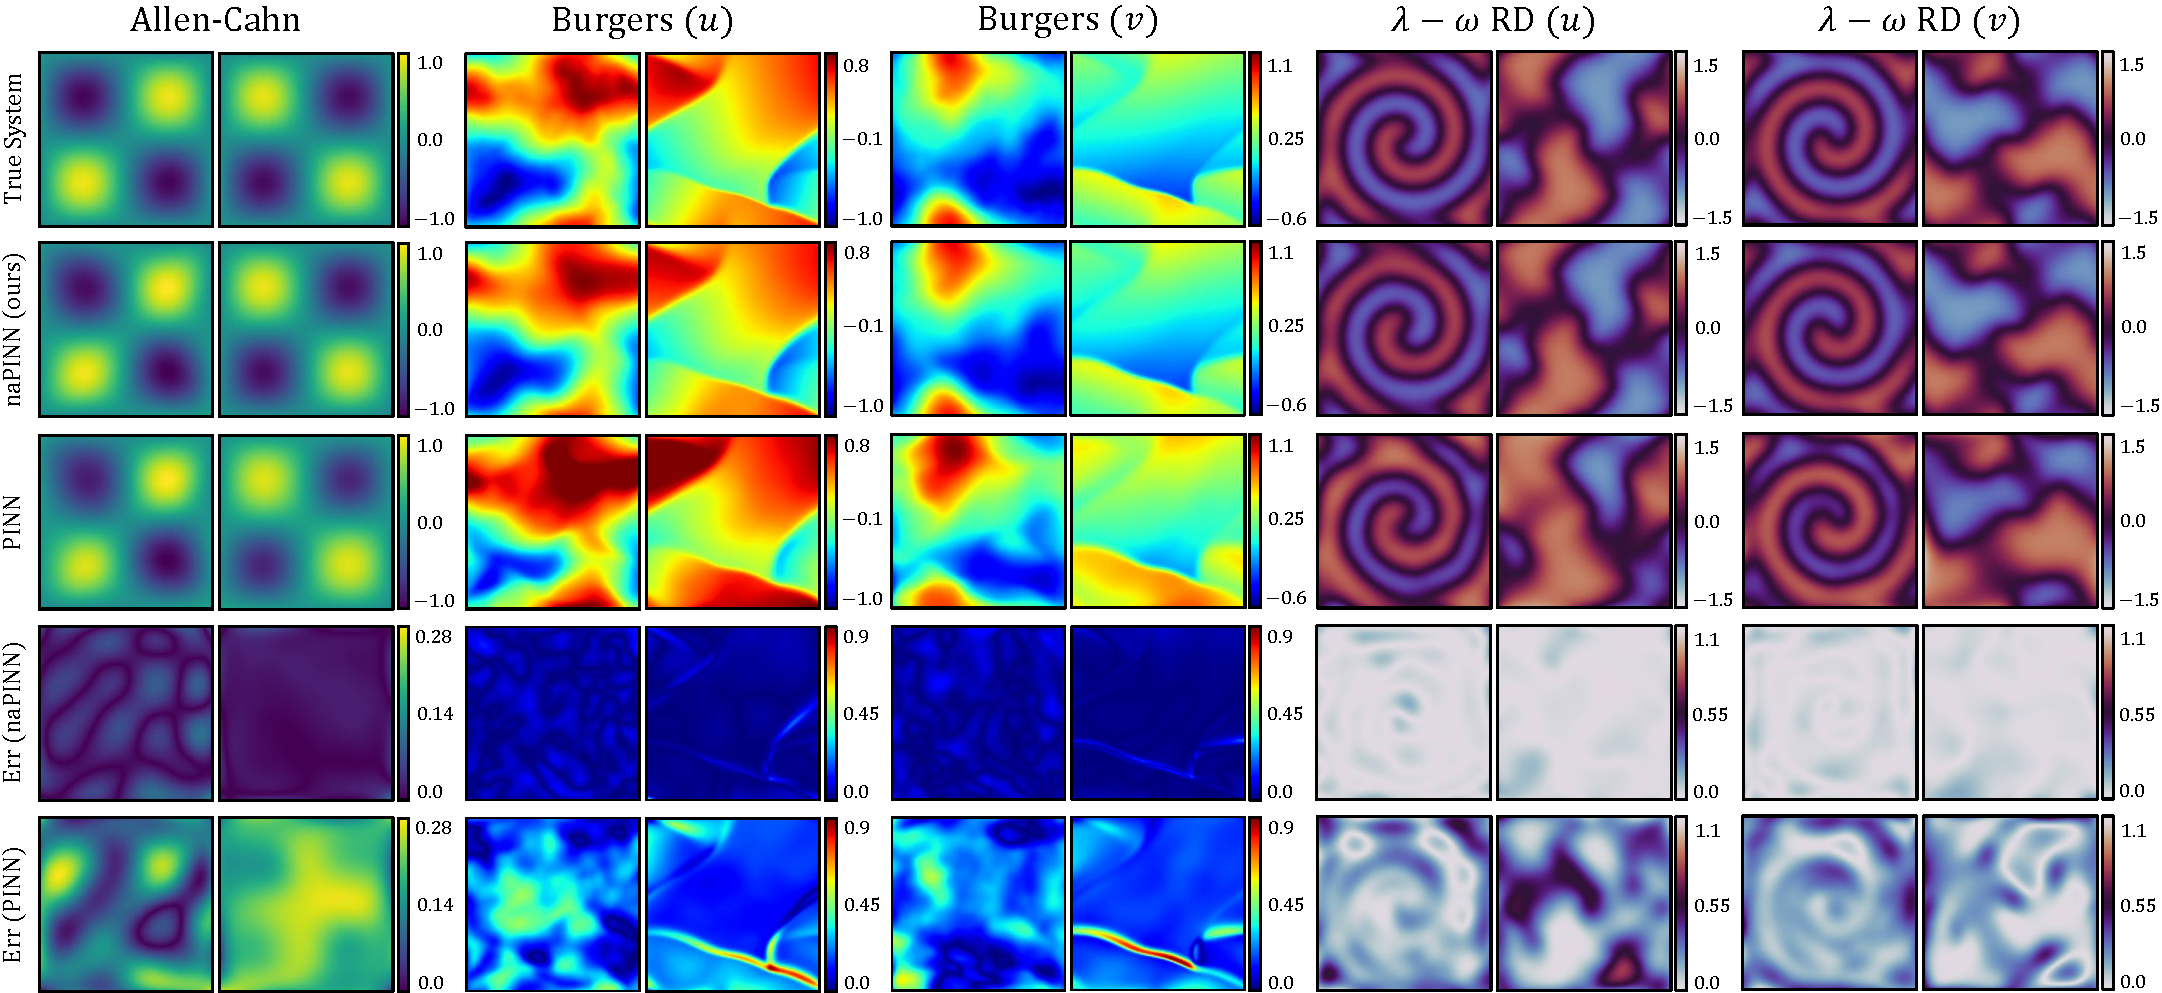
\includegraphics[width=0.92\textwidth]{figures/qualitative.pdf}
\caption{Reconstructions under $10\%$ gross outliers at two time slices per
field. The rows show the reference solution, naPINN, a standard PINN, and the
absolute errors of naPINN and of the standard PINN. Color scales differ across
fields.}
\label{fig:qualitative}
\end{figure*}


\paragraph{Simulated benchmarks.}
We use three PDEs in two space dimensions and time, each with one unknown
coefficient. These are Allen--Cahn with interface width $\varepsilon$, Burgers
with viscosity $\nu$, and a $\lambda$--$\omega$ reaction--diffusion system with
reaction parameter $\beta$. Reference solutions solve the same equations that
the PDE residual enforces, so the residual has no model discrepancy. Sensors are
placed on a fixed $15 \times 15$ spatial grid and record at every time step.
Measurements are corrupted by an asymmetric four-component Gaussian-mixture
background noise. In addition, $5\%$, $10\%$ or $15\%$ of the measurement rows,
each holding all components recorded by one sensor at one time, receive a
positive gross offset $c\,\sigma_\epsilon$ with $c \sim \mathcal{U}(3,10)$, where
$\sigma_\epsilon$ is the background standard deviation (\cref{app:benchmarks}).

\paragraph{Real measurements.}
We use time-resolved PIV of flow past a cylinder from RealPDEBench
\citep{hu2026realpdebench}, with $200$ frames at $192$ fixed, irregularly placed
training sensors. Evaluation uses held-out PIV vectors at locations disjoint
from the training sensors (\cref{app:real}). Only the training sensors are
corrupted, using the same generator as for the simulated benchmarks at $10\%$
and $15\%$ of rows. The corruption
intensity was fixed before any run and never tuned. We treat the held-out PIV
as an independent measurement rather than noise-free truth. The forward model
is a nominal two-dimensional incompressible Navier--Stokes residual with a
latent pressure field. It only approximates the real flow, so the residuals
contain model discrepancy as well as sensor error. The Reynolds number is held
at its metadata value, so no coefficient is estimated and all real-PIV results
measure field reconstruction.

\paragraph{Methods.}
All methods share the same backbone, an MLP with five $\tanh$ hidden layers of
width $80$, as well as the optimizer and the $30{,}000$-update PINN budget,
except for MAD-PINN and the wall-clock-matched control. The
fixed-loss baselines are PINN (MSE), LAD-PINN \citep{Peng2022} and OrPINN with
$q = 1.9$ and $q = 2.9$ \citep{Duarte2025}. B-PINN is the mean-field variational
version, not the HMC sampler of \citet{Yang2021} (\cref{app:notrun}). PINN-EBM
\citep{Pilar2024} shares naPINN's estimator, staged initialization and budget.
We swept its $\wpde$ over $\{1, 10, 50\}$ and report the setting with the
lowest rMAE, $\wpde = 10$ on the simulated benchmarks and $\wpde = 50$ on real
PIV, while all other methods use $\wpde = 1$ (\cref{app:pinnebm}).
Screening baselines and MAD-PINN are described in \cref{sec:mechanism}, and a
wall-clock-matched control in \cref{sec:exact}.

naPINN uses the EBM estimator,
$\wpde = 1$, $\rej = 0.5$ and gate parameters initialized at $\tilde\tau = 2$
and $\tilde a = 30$ on every benchmark and on real PIV, and none of these values was tuned per problem.
naPINN uses the standard squared loss in all main comparisons. We test it in this
most common setting instead of choosing a loss with prior knowledge of the
noise, so any advantage over the robust losses comes from the adaptive
weighting. We report combinations of naPINN with an $\ell_1$ loss
(naPINN-L1) and a $q$-Gaussian loss (naPINN-$q$2.9) separately.

\paragraph{Metrics.}
In both settings we report the relative mean absolute error (rMAE) and the
relative $L_2$ error (rMSE) of the field, on a $120 \times 120$ spatial grid for
the simulated benchmarks and at the held-out locations for real PIV
(\cref{app:benchmarks}).

\paragraph{Trials and seeds.}
The simulated-benchmark results come from two sets of experiments.
\Cref{tab:exact} uses ten trials at every outlier ratio, while the ablation
study (\cref{tab:mechanism}), the coefficient errors, the sensitivity studies
and the compute controls use a later set of three seeds
(seeds $40$--$42$) at $15\%$
(\cref{app:repro}). Each table compares methods within one set, and real-PIV
results use seeds $40$--$42$. At $15\%$, naPINN's three-seed values differ from
its ten-trial values by less than the ten-trial standard deviations.

% ====================================================================
\section{RESULTS}
\label{sec:results}





\subsection{Simulated Benchmarks}
\label{sec:exact}

\Cref{tab:exact} reports all three outlier ratios. Against the fixed losses,
naPINN's rMAE at $15\%$ outliers is lower than that of the best robust-loss
baseline, OrPINN ($q = 2.9$), by a factor of $2.0$, $2.4$ and $2.0$, and the
variational B-PINN does not improve on MSE. Both methods that learn the noise
distribution have lower error than every fixed loss at every outlier ratio, and
PINN-EBM is the strongest comparator. naPINN has lower rMAE than PINN-EBM in
seven of the nine settings. On Allen--Cahn at $5\%$ PINN-EBM is lower by
$0.001$, and on Burgers at $5\%$ the two tie. In all Allen--Cahn and Burgers
settings and on $\lambda$--$\omega$ at $5\%$, the difference is smaller than the
larger of their two standard deviations, whereas on $\lambda$--$\omega$ at
$10\%$ and $15\%$ naPINN's rMAE is $19\%$ and $27\%$ lower.

naPINN's error stays nearly flat as the outlier ratio grows from $5\%$ to $15\%$,
with its rMAE changing by at most $0.03$, whereas every fixed loss degrades steadily (\cref{fig:ratio_curve}). The reconstructed
fields in \cref{fig:qualitative} show the same difference from a standard PINN.
naPINN recovers the Allen--Cahn field structure, the Burgers shock and the
$\lambda$--$\omega$ spiral, while the ungated PINN shows broad amplitude errors
and an error ridge along the Burgers shock.

A wall-clock-matched control gives the same ordering. When each fixed-loss
baseline trains for as long as naPINN in wall-clock time, which allows on
average $37{,}561$ to $53{,}494$ updates depending on the baseline and
benchmark, the best of them, OrPINN ($q = 2.9$), still has at least $1.9$ times
the error of naPINN (\cref{app:compute}).

\paragraph{Coefficient recovery.}
We also measure how accurately each method recovers the unknown coefficients
(\cref{app:exact}, three-seed experiments). naPINN and PINN-EBM recover all
three coefficients with similar accuracy at $15\%$ outliers. Their relative
errors are $0.9\%$, $7.2\%$ and $1.4\%$ for naPINN and $0.7\%$, $6.5\%$ and
$1.0\%$ for PINN-EBM on $\varepsilon$, $\nu$ and $\beta$. The fixed losses are less accurate, with
at least $12\%$ error on $\nu$ and $5\%$ on $\beta$. The small viscosity $\nu$
is the hardest coefficient for every method.

\subsection{Real Measurements Under a Nominal PDE}
\label{sec:real}

\begin{table}[t]
\centering
\caption{Held-out rMAE\,/\,rMSE on real PIV (RealPDEBench Cylinder) with $10\%$
and $15\%$ corrupted training rows, mean over seeds $40$--$42$. All eight
methods, with standard deviations, are reported in \cref{app:real}. Best in
bold, second best underlined.}
\label{tab:piv}
\vspace{4pt}
\small
\setlength{\tabcolsep}{3pt}
\begin{tabular}{lcc}
\toprule
Method & $10\%$ & $15\%$ \\
\midrule
PINN (MSE)                 & 0.406\,/\,0.429 & 0.574\,/\,0.591 \\
LAD-PINN                   & 0.246\,/\,0.278 & 0.270\,/\,0.300 \\
OrPINN ($q = 2.9$)           & \underline{0.214}\,/\,\underline{0.250} & \underline{0.231}\,/\,\underline{0.265} \\
PINN-EBM ($\wpde = 50$)   & 0.224\,/\,0.331 & 0.336\,/\,0.414 \\
\textbf{naPINN}            & \textbf{0.155}\,/\,\textbf{0.215} & \textbf{0.160}\,/\,\textbf{0.223} \\
\bottomrule
\end{tabular}
\vspace{-14pt}
\end{table}

On real PIV (\cref{tab:piv}), naPINN has the lowest held-out rMAE and rMSE at
both corruption levels among the eight methods run, and it is lowest on each of
the three seeds. Its rMAE is $28\%$ and $31\%$ lower than that of the best baseline,
OrPINN ($q = 2.9$). The gate also separates corrupted from clean measurements
on real data. It excludes $98.99\%$ and $99.23\%$ of the corrupted measurement
components but only $2.95\%$ and $4.23\%$ of the clean ones. Combinations of naPINN with robust losses are
reported in \cref{app:real}.

On three other RealPDEBench scenarios (Controlled Cylinder, FSI and Foil),
planned before any run, naPINN has
the lowest mean rMAE in all six conditions and the lowest mean rMSE in four of
them, with OrPINN ($q = 2.9$) lowest in rMSE on FSI at both levels
(\cref{app:real}).

The gap to PINN-EBM is larger on real data. On the simulated benchmarks
naPINN's rMAE is at most $19\%$ and $27\%$ lower than that of PINN-EBM at $10\%$
and $15\%$ outliers, against $31\%$ and $52\%$ on real PIV, where PINN-EBM also
has higher error than both fixed robust losses at $15\%$. On real data the learned density
must absorb model discrepancy as well as sensor error. A possible reason for the
widening is that PINN-EBM uses the derivative of the learned log-density in
every update, so errors in the density's shape enter the fit directly, whereas
naPINN uses the density only through detached, standardized scores that set
per-measurement weights. Because the two regimes also
differ in data source, sensor layout and evaluation target, we report the
widening as an association.

\begin{table}[t]
\centering
\caption{Field rMAE in the ablation study at $15\%$ gross outliers,
mean\,$\pm$\,s.d.\ over seeds $40$--$42$. The first row is naPINN. A fixed gate
is frozen at initialization for the density and set to the minibatch $95\%$
quantile for $|\tilde r|$. MAD-PINN uses $60{,}000$ updates and all other rows
$30{,}000$. Best in bold, second best underlined.}
\label{tab:mechanism}
\vspace{4pt}
\small
\setlength{\tabcolsep}{3pt}
\resizebox{\columnwidth}{!}{%
\begin{tabular}{llccc}
\toprule
Ordering & Gate & Allen--Cahn & Burgers & $\lambda$--$\omega$ \\
\midrule
\multicolumn{5}{l}{\emph{Selection during training}} \\
density & learned & \textbf{0.092}\sd{0.004} & \textbf{0.082}\sd{0.002} & \textbf{0.071}\sd{0.001} \\
density & fixed   & 0.675\sd{0.162} & 0.514\sd{0.067} & 0.351\sd{0.016} \\
$|\tilde r|$ & learned & 0.244\sd{0.039} & 0.345\sd{0.014} & 0.148\sd{0.011} \\
$|\tilde r|$ & fixed   & 0.509\sd{0.159} & 0.373\sd{0.031} & 0.237\sd{0.009} \\
\midrule
\multicolumn{5}{l}{\emph{Pre-training screen, then PINN (MSE)}} \\
\multicolumn{2}{l}{global $z$-score}  & 0.449\sd{0.060} & 0.207\sd{0.003} & 0.156\sd{0.018} \\
\multicolumn{2}{l}{global MAD}        & 0.321\sd{0.029} & 0.161\sd{0.016} & 0.096\sd{0.002} \\
\multicolumn{2}{l}{neighborhood median} & \underline{0.152}\sd{0.078} & \underline{0.121}\sd{0.017} & \underline{0.083}\sd{0.005} \\
\midrule
\multicolumn{2}{l}{MAD-PINN (two-stage)} & 0.344\sd{0.043} & 0.242\sd{0.012} & 0.127\sd{0.006} \\
\bottomrule
\end{tabular}%
}
\end{table}

\begin{figure*}[t]
\centering
\begin{minipage}[t]{0.48\textwidth}
  \centering
  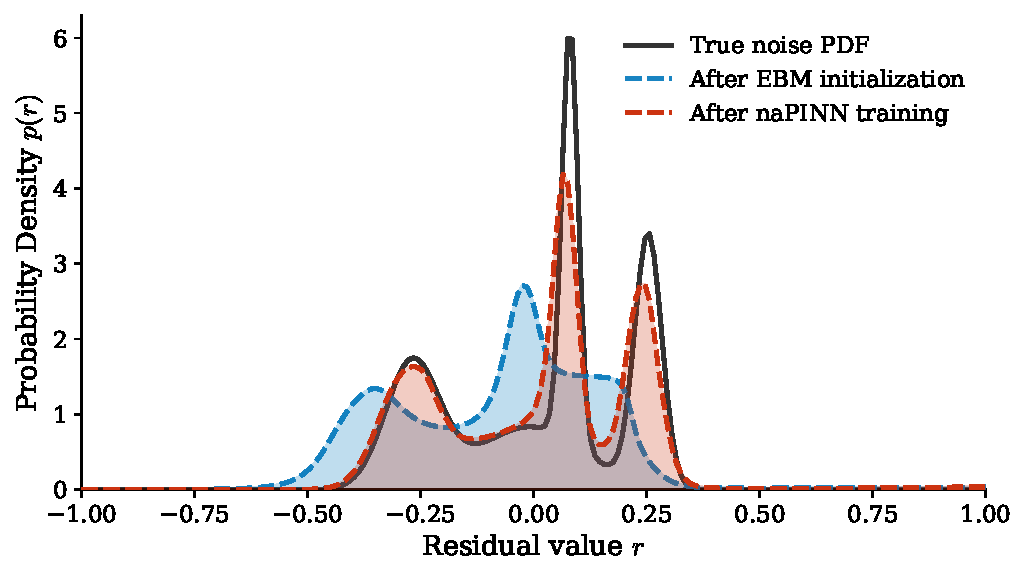
\includegraphics[width=\linewidth]{figures/noise_pdf.pdf}
\end{minipage}\hfill
\begin{minipage}[t]{0.48\textwidth}
  \centering
  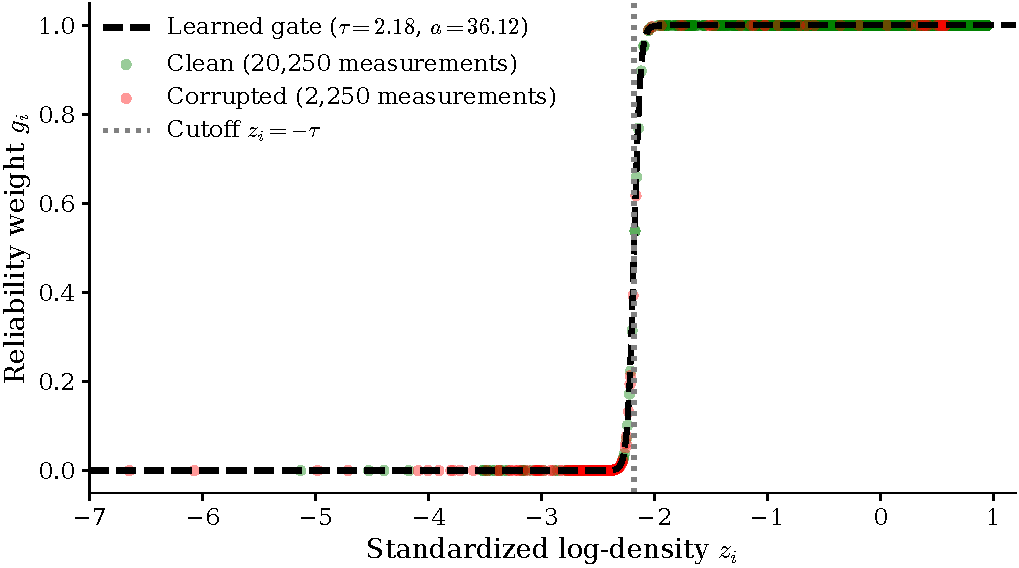
\includegraphics[width=\linewidth]{figures/gate.pdf}
\end{minipage}
\caption{\textbf{Left.} Learned residual density after estimator initialization
and after joint training, against the injected background-noise density
(Burgers, $5\%$ gross outliers). Joint training resolves the asymmetric,
multimodal noise. \textbf{Right.} Trained gate against the standardized
log-density on Allen--Cahn at $10\%$ gross outliers, with one in five
measurements of each class plotted. The gate is nearly a hard decision and
excludes $98\%$ of corrupted and $0.75\%$ of clean measurements. Labels are used
only for this plot.}
\label{fig:learned}
\end{figure*}

\subsection{Ablation Study}
\label{sec:mechanism}

The top block of \cref{tab:mechanism} changes two parts of naPINN
independently. The gate orders measurements either by their learned
log-density or by their normalized residual magnitude $|\tilde r|$, and its
parameters (cutoff and steepness) are either trained or fixed. All four
combinations use the same sigmoid gate, and the first row is naPINN.

\paragraph{Learning the gate.}
To test whether the gate must be learned, we keep the learned density and
freeze the gate at its initialization. This changes only whether the gate is
trained (\cref{app:ablations}) and raises rMAE to $0.675$, $0.514$ and $0.351$
(\cref{tab:mechanism}). The frozen
gate excludes $20.9$--$28.3\%$ of the corrupted components, compared with
$99.3$--$99.4\%$ for the trained gate, while clean-data exclusion stays similar
($0.5$--$1.3\%$ against $0.7$--$1.1\%$). The learned density already orders the
measurements well, but the gate has to be learned before it excludes the
corrupted ones.

\paragraph{Ordering by density.}
To test whether the ordering must come from the learned density, we train the
same gate on the normalized residual magnitude $|\tilde r|$ with the same
rejection cost. This selector is close to the trimmed estimator in
\cref{prop:gate}(a), and its rMAE is more than twice that of naPINN. A fixed $95\%$ quantile of $|\tilde r|$ is worse
still. Read as a hard threshold it excludes about $5\%$ of the measurements, so
under $15\%$ corruption it cannot exclude more than a third of the outliers. We attribute the advantage of
ordering by density to the asymmetric, multimodal background noise
(\cref{fig:learned}, left), under which typical residuals need not lie near zero.

\paragraph{Pre-training screens.}
We also compare with three screens that remove suspicious measurements before
training, using thresholds tuned on the true corruption labels. Global $z$-score and MAD rules applied to raw values do not distinguish
a corrupted measurement from a legitimate extremum of a field that varies in
space and time, so their errors are at least $1.3$ times that of naPINN. A neighborhood-median rule avoids this and detects almost all
outliers, yet it still has higher error than naPINN on all three benchmarks and
a seed spread $5$--$20$ times larger, which we attribute to the remaining
outliers entering an unweighted loss. The two-stage MAD-PINN \citep{Peng2022},
which uses twice the update budget, also discards $10.6$--$19.0\%$ of the clean
data and has higher error than naPINN on all three benchmarks
(\cref{app:screens}).

\subsection{Modularity and Sensitivity}
\label{sec:practical}
Because naPINN only reweights the data loss, it can be added to different PINN
models, and its own components can be exchanged. With
the MLP and with four other backbones (KAN, FLS, QRes and PirateNet), naPINN
reduces the error of the plain PINN by a factor of at least $3$ for
every benchmark at $10\%$ outliers (\cref{app:backbone}). A Gaussian
mixture or a kernel density estimate can replace the EBM. Both give accuracy
similar to the EBM, better on Allen--Cahn at some outlier ratios and no better
on Burgers or $\lambda$--$\omega$ (\cref{app:ablations}). Under purely Laplace or Gaussian
background noise, naPINN with the squared loss does not beat LAD-PINN or OrPINN,
but naPINN combined with an $\ell_1$ loss beats both (\cref{app:ablations}). The
loss that works best inside naPINN depends on the noise.

Changing the running-scale weight $m$ from $0.01$ to $0.10$ changes the error
by less than the variation across seeds, and accuracy is stable for
$\rej \in [0.1, 0.8]$. Removing the rejection cost increases the error, and the
error rises sharply for $\rej \ge 0.9$, consistent with \cref{prop:gate}(b). A sharper
initial gate ($\tilde a = 60$) diverged on one of three seeds (\cref{app:sensitivity}).

% ====================================================================
\section{DISCUSSION}
\label{sec:discussion}

naPINN gives the lowest field error in nearly all simulated settings and on
real PIV, and in our ablations neither the learned residual density nor the
trainable gate suffices on its own. Its per-measurement weights also identify
corrupted measurements with high accuracy. Because every measurement receives
an explicit reliability weight, naPINN can serve not only to recover physics
from corrupted data but also as an anomaly detector for measurements of systems
governed by a PDE. Future work includes identifying PDE coefficients from real
measurements and applying naPINN to other sensor-driven systems governed by
PDEs, such as subsurface flow and environmental monitoring networks, where
locating faulty sensors is valuable in itself.

\subsection*{AI use statement}
In this work, we used generative AI tools to assist with writing and editing
the manuscript text and with implementing and checking experiment and analysis
code. We did not use generative AI tools to generate research ideas or
experimental data. We have reviewed all AI-assisted work, verified
AI-assisted code by running it, and checked every reported number against our
experiment records. We take responsibility for the final content of this work,
including text, claims, or artifacts produced with the aid of generative AI.

\bibliographystyle{plainnat}
\bibliography{references}

% ====================================================================
\clearpage
\appendix
\thispagestyle{empty}
\onecolumn
\aistatstitle{naPINN: Noise-Adaptive Physics-Informed Neural Networks \\
for Recovering Physics from Corrupted Measurements \\ Supplementary Materials}

\section{PROOF OF PROPOSITION 1}
\label{app:proof}

Throughout, the standardized log-densities $z_i$, including the minibatch
statistics $\mu_\ell$ and $\sigma_\ell$, are computed without gradient, as in
\cref{eq:gate} and the implementation. Hence $g_i$ depends on the trainable
parameters only through $\tilde a$ and $\tilde\tau$, and $r_i$ depends only on
$\theta$ and $\boldsymbol\eta$. Write
$\mathcal{L}_g = \mathcal{L}_{\mathrm{data}} + \rej\mathcal{L}_{\mathrm{rej}}
= \frac{1}{N_d}\sum_i h(g_i, r_i)$ with $h(g, r) = g\,r^2 + \rej(1-g)$.

\textbf{(a)} For fixed $r$, $h(g, r) = \rej + g\,(r^2 - \rej)$ is affine in $g$.
On $[0,1]$ it is minimized at $g = 1$ if $r^2 < \rej$, at $g = 0$ if
$r^2 > \rej$, and by every $g$ if $r^2 = \rej$. The minimum is $r^2$ in the first
case and $\rej$ in the second, that is $\min\{r^2, \rej\}$. The measurements
decouple once the gates are free, so minimizing $\mathcal{L}_g$ over the gates
gives the trimmed loss.

\textbf{(b)} With $\tau = \softplus(\tilde\tau)$ and $g_i = \sig(a(z_i+\tau))$,
$\partial g_i/\partial\tilde\tau = a\, g_i(1-g_i)\,\softplus'(\tilde\tau)$, using
$\sig' = \sig(1-\sig)$. By the chain rule and $\partial h/\partial g = r^2 - \rej$,
$\partial\mathcal{L}_g/\partial\tilde\tau =
\frac{a\,\softplus'(\tilde\tau)}{N_d}\sum_i g_i(1-g_i)(r_i^2 - \rej)$, which is the
stated expression with $c = a\,\softplus'(\tilde\tau)/N_d$. Since
$a > 0$ and $\softplus' > 0$, a stationary point requires
$\sum_i g_i(1-g_i)\, r_i^2 = \rej \sum_i g_i(1-g_i)$, which is the stated
weighted mean whenever $\sum_i g_i(1-g_i) > 0$. The same computation for the
steepness gives $\partial\mathcal{L}_g/\partial\tilde a =
\frac{\softplus'(\tilde a)}{N_d}\sum_i g_i(1-g_i)(z_i + \tau)(r_i^2 - \rej)$.

\textbf{(c)} Let $\delta_i = z_i + \tau$. Since $\sigma_\ell > 0$,
$\delta_i > 0$ exactly when $\ell_\phi(\tilde r_i) > \mu_\ell - \tau\sigma_\ell$.
For $\delta_i \neq 0$, $\sig(a\,\delta_i) \to \mathbf{1}\{\delta_i > 0\}$ as
$a \to \infty$, which gives the stated limit. The set
$\{\tilde r : \ell_\phi(\tilde r) > \mu_\ell - \tau\sigma_\ell\}$ is
a superlevel set of $p_\phi$. If $\ell_\phi$ is symmetric about zero and strictly
decreasing in $|\tilde r|$, it equals $\{|\tilde r| < r_0\}$ for some $r_0$.
For general asymmetric or multimodal densities, superlevel sets need not be
intervals centered at zero.
\hfill$\square$

\section{IMPLEMENTATION DETAILS}
\label{app:method}



\paragraph{Estimators.}
All estimators share one interface. They receive the normalized scalar residuals
$\tilde r_i$ (multi-output residuals flattened) and return a log-density for
each. The PINN, optimizer, schedule, batches, normalization and gate are
identical across estimators.
\begin{itemize}
\item \emph{EBM (main).} A $\tanh$ MLP with three hidden layers (two on real PIV) of width $32$
maps $\tilde r$ to a scalar, the log-density up to a constant. The
log-partition function is approximated by trapezoidal integration on a fixed
grid over $[-10, 10]$ ($1{,}024$ points on the simulated benchmarks). It is
trained by maximum likelihood on detached residuals with Adam, learning rate
$10^{-3}$.
\item \emph{Gaussian mixture.} Three components (the estimator is not told that
the background noise has four) with trainable
logits, means and log standard deviations, means initialized near zero,
trained by maximum likelihood with Adam, learning rate $10^{-2}$.
\item \emph{Kernel density estimate.} A Gaussian kernel over a buffer of up to
$2{,}048$ recent normalized residuals, with Silverman bandwidth
$h = 0.9\min(s, \mathrm{IQR}/1.34)\,n^{-1/5}$ clamped from below. It has no
trainable parameters, and each step refreshes the buffer and bandwidth.
\end{itemize}

\paragraph{Gate.}
The trainable variables are the pre-softplus values $\tilde a$ and $\tilde\tau$,
initialized at $\tilde a = 30$ ($a \approx 30$) and $\tilde\tau = 2$
($\tau \approx 2.13$). The gate therefore starts by excluding only measurements
about two standard deviations below the mean log-density, which avoids early
mass rejection. The rejection term is averaged over the minibatch.

\paragraph{Architecture and optimization.}
The implementation uses PyTorch. All methods use Adam with learning rate
$10^{-3}$ for the network, the unknown coefficient and the gate parameters (the
Gaussian mixture uses $10^{-2}$), with no learning-rate schedule and no weight
decay. Each update samples collocation points and measurement rows with
replacement, with the sizes below, and the running scale is clipped from below
at $10^{-6}$. The PINN is a five-hidden-layer
$\tanh$ MLP of width $80$ mapping space--time coordinates to one field (Allen--Cahn), two
fields (Burgers, $\lambda$--$\omega$), or velocity plus latent pressure (real
PIV). The PDE and data terms both have weight one for all methods except PINN-EBM
(\cref{app:pinnebm}), and no boundary or initial-condition loss is used.

\begin{center}\small
\setlength{\tabcolsep}{6pt}
\begin{tabular}{lcccc}
\toprule
 & Allen--Cahn & Burgers & $\lambda$--$\omega$ & Real PIV \\
\midrule
collocation points per update & $5{,}000$ & $5{,}000$ & $10{,}000$ & $8{,}192$ \\
measurement rows per update    & $1{,}000$ & $1{,}000$ & $2{,}000$ & $2{,}048$ \\
EBM hidden layers / quadrature points & $3$ / $1{,}024$ & $3$ / $1{,}024$ & $3$ / $1{,}024$ & $2$ / $256$ \\
\bottomrule
\end{tabular}
\end{center}

\paragraph{Residual normalization.}
The running scale uses weight $m = 0.05$ on the new minibatch statistic,
equivalently decay $0.95$ on the old state. Recomputing the scale from each
minibatch instead, with no smoothing, is worse in eight of nine cells of the
ten-trial experiments (rMSE).

\begin{center}\small
\begin{tabular}{llccc}
\toprule
Benchmark & Normalization & $5\%$ & $10\%$ & $15\%$ \\
\midrule
\multirow{2}{*}{Allen--Cahn}
 & running & \textbf{0.101} & \textbf{0.108} & \textbf{0.127} \\
 & per-batch & 0.182 & 0.141 & 0.200 \\
\midrule
\multirow{2}{*}{Burgers}
 & running & 0.089 & \textbf{0.092} & \textbf{0.091} \\
 & per-batch & \textbf{0.086} & 0.101 & 0.111 \\
\midrule
\multirow{2}{*}{$\lambda$--$\omega$}
 & running & \textbf{0.092} & \textbf{0.092} & \textbf{0.095} \\
 & per-batch & 0.105 & 0.096 & 0.098 \\
\bottomrule
\end{tabular}
\end{center}

\paragraph{Latent-variable reading.}
The gate can be read as an inclusion responsibility, although \cref{eq:total}
is not the likelihood of the density estimator. Introduce an indicator
$c_i \in \{0,1\}$ and a Gaussian model for included measurements,
$p_\theta(y_i \mid \mathbf{x}_i, t_i, c_i{=}1) =
\mathcal{N}(\hat u_\theta(\mathbf{x}_i, t_i), \sigma_y^2)$. Under
$q(c_i{=}1) = g_i$ the expected included-data negative log-likelihood is, up to
constants, $(2\sigma_y^2)^{-1}\sum_i g_i r_i^2$. Here $g_i$ plays the role of a
responsibility, with the learned log-density $\ell_\phi$ determining it. The
linear rejection term is an explicit price on exclusion.

\section{BENCHMARK DETAILS}
\label{app:benchmarks}

Each benchmark has one unknown coefficient, which is trained jointly with the
network from an initial value far from the truth. Boundary and initial
conditions do not enter the loss and are used only to generate the reference
solution.

Throughout this section $(x, y)$ are spatial coordinates.

\paragraph{Allen--Cahn.}
$u_t - \varepsilon^2 \Delta u + (u^3 - u) = f(x,y,t)$ on $[0,2]^2 \times [0,2]$,
with the manufactured solution $u^* = \sin(\pi x)\sin(\pi y)\cos(\omega t)$ with temporal
frequency $\omega = 8$ and
the forcing $f = u^*_t - \varepsilon^2\Delta u^* + (u^*)^3 - u^*$ it implies, so
$u^*$ satisfies the PDE exactly. The true interface width is
$\varepsilon = 0.3$, and training starts from $\varepsilon = 1.0$.

\paragraph{Burgers.}
$u_t + u u_x + v u_y = \nu \Delta u$ and $v_t + u v_x + v v_y = \nu \Delta v$ on
$[0,4]^2$, recorded over $T = 3.0$ after a discarded burn-in of $0.1$. Both
velocity components are initialized from Gaussian random fields with spectral
decay $\alpha = 5.0$, which gives smooth but spatially diverse initial
conditions and turbulence-like dynamics. The reference is computed with
second-order central differences and explicit Euler time stepping under a monitored
viscous CFL condition. The true viscosity is $\nu = 0.01$, and training starts from
$\nu = 0$.

\paragraph{$\lambda$--$\omega$ reaction--diffusion.}
$u_t = d_u \Delta u + \lambda(A)u - \omega(A)v$ and
$v_t = d_v \Delta v + \omega(A)u + \lambda(A)v$ with $A^2 = u^2 + v^2$,
$\lambda(A) = 1 - A^2$ and $\omega(A) = -\beta A^2$, on
$[-10,10]^2 \times [0,10]$ with periodic boundaries and $d_u = d_v = 1$. The
initial state is a spiral,
$u = s\cos(\vartheta - s)$, $v = s\sin(\vartheta - s)$ with
$s = \tanh\sqrt{x^2+y^2}$ and $\vartheta = \arg(x + iy)$, and the reference is
computed with the same finite-difference scheme. The true coefficient is
$\beta = 1.0$, and training starts from $\beta = 0$.

\paragraph{Sensors and corruption.}
Sensors lie on a fixed $15 \times 15$ spatial grid and record at every time
step, and collocation points are drawn from a $100 \times 100$ spatial grid. The
background noise is an equal-weight mixture of four Gaussians with (mean,
standard deviation) $(-9, 2)$, $(-0.3, 4)$, $(2.7, 0.6)$ and $(8.5, 1.0)$,
multiplied by $0.1$ times the mean absolute value of the clean field. It is
asymmetric and multimodal. A fraction of $5\%$, $10\%$ or $15\%$ of measurement
rows then receives an additive offset $c\,\sigma_\epsilon$ on every component,
with $c \sim \mathcal{U}(3,10)$ drawn independently and $\sigma_\epsilon$ the
standard deviation of the background noise. The corruption labels are stored
for diagnosis only.

\paragraph{Why simulated benchmarks.}
Generating measurements from a known reference (a twin experiment) is the
standard way to measure reconstruction error, coefficient error and corruption
severity under control \citep{Asch2016}, and it is how prior robust-PINN work
is evaluated \citep{Yang2021, Peng2022, Duarte2025}. We know of no public
benchmark that provides sparse corrupted sensor data together with a governing
PDE, a clean reference, an unknown coefficient and corruption labels. The real
PIV experiments complement this with measurements whose noise and model
discrepancy we did not design.

\paragraph{Metrics.}
For a field with $K$ components evaluated at the grid points and evaluation
times $j = 1,\dots,M$, with $\mathbf{e}_j = \hat{\mathbf{u}}_j - \mathbf{u}_j \in
\mathbb{R}^K$,
\begin{equation*}
\mathrm{rMAE} = \frac{\frac{1}{M}\sum_j \|\mathbf{e}_j\|_2}{\frac{1}{M}\sum_j
\|\mathbf{u}_j\|_2}, \qquad
\mathrm{rMSE} = \frac{\big(\frac{1}{M}\sum_j \|\mathbf{e}_j\|_2^2\big)^{1/2}}
{\big(\frac{1}{M}\sum_j \|\mathbf{u}_j\|_2^2\big)^{1/2}},
\end{equation*}
which for $K = 1$ are the usual scalar relative errors. The
simulated benchmarks are evaluated on a $120 \times 120$ spatial grid, finer
than the collocation grid, and real PIV is evaluated at the held-out sensor
locations.

\section{BASELINE DETAILS}
\label{app:baselines}

All baselines share the MLP backbone (five $\tanh$ hidden layers of width $80$,
Xavier-uniform weights, zero biases), the optimizer and the update budget,
except for MAD-PINN.

\paragraph{Data losses.} PINN and naPINN use the MSE $\rho(r_i) = r_i^2$, the
Gaussian negative log-likelihood. LAD-PINN uses $\rho(r_i) =
|r_i|$, the Laplace negative log-likelihood with fixed scale. OrPINN \citep{Duarte2025} uses the
$q$-Gaussian negative log-likelihood
$\rho_q(r_i) = \frac{1}{q-1}\log\!\big(1 + (q-1)\beta_q r_i^2\big)$ with
$\beta_q = 1/(2(3-q))$, a scale convention that recovers a quadratic loss as
$q \to 1$. We report $q = 1.9$ and $q = 2.9$, which give heavy-tailed losses
whose densities have no finite variance.

\paragraph{Variational B-PINN.} Every linear layer of the MLP is replaced by a
Bayesian layer with a factorized Gaussian posterior and a $\mathcal{N}(0,1)$
prior. Training samples one weight draw per update by the reparameterization
trick and adds the KL divergence with weight $10^{-6}$. Evaluation uses the
posterior mean.

\paragraph{PINN-EBM.}
\label{app:pinnebm}
Following \citet{Pilar2024}, a one-dimensional EBM is trained jointly with the
PINN, and its negative log-likelihood of the normalized residuals is the data
loss. Gradients flow into the PINN, the EBM and the unknown coefficient, and
there is no gate or rejection cost. The EBM architecture, the staged
initialization and the $30{,}000$-update PINN budget are the same as for
naPINN. All other methods use $\wpde = 1$ without tuning. For PINN-EBM the
balance between a likelihood data term and the PDE residual does not transfer
across problems, so we swept $\wpde \in \{1, 10, 50\}$ on its behalf. On the
simulated benchmarks \cref{tab:exact} reports the setting with the lowest
rMAE, $\wpde = 10$, at every outlier ratio. On real PIV at $15\%$ corrupted rows, $\wpde = 1$ gives
held-out rMAE\,/\,rMSE of $0.424$\,/\,$0.464$, worse than the
$0.336$\,/\,$0.414$ of $\wpde = 50$, so \cref{tab:piv} reports $\wpde = 50$. The
comparison contrasts two uses of the same estimator and is not a one-factor
ablation.

\paragraph{Two-stage MAD-PINN.}
Following \citet{Peng2022}, it runs $30{,}000$ LAD updates, the published fixed screen
$|r| > 3\,\mathrm{median}(|r|)/1.6777$, then $30{,}000$ MSE updates on the
retained components, initialized from the first stage. It uses twice the update
budget and is a reference rather than a compute-matched peer.

\paragraph{HMC B-PINN.}
\label{app:notrun}
A faithful HMC Bayesian PINN \citep{Yang2021} needs a specified prior, step-size
and trajectory schedule, burn-in, sample budget and convergence diagnostics over
a posterior over the $26{,}402$ network parameters. We implemented one and could not
establish convergence, so we report no number from it and make no claim relative
to HMC B-PINNs. The variational B-PINN in \cref{tab:exact} uses a factorized
Gaussian posterior, a weaker approximation. Bayesian treatment of the weights is
orthogonal to the inclusion decision studied here, and the two could be
combined.

\section{ADDITIONAL RESULTS ON SIMULATED BENCHMARKS}
\label{app:exact}

\paragraph{Robustness across outlier ratios.}
\Cref{fig:ratio_curve} plots the rMSE of \cref{tab:exact} against the outlier
ratio. The fixed
losses degrade roughly linearly with the outlier ratio, while naPINN is nearly
flat between $5\%$ and $15\%$, as expected if corrupted measurements are
excluded rather than downweighted by a fixed penalty.



\begin{figure}[h]
\centering
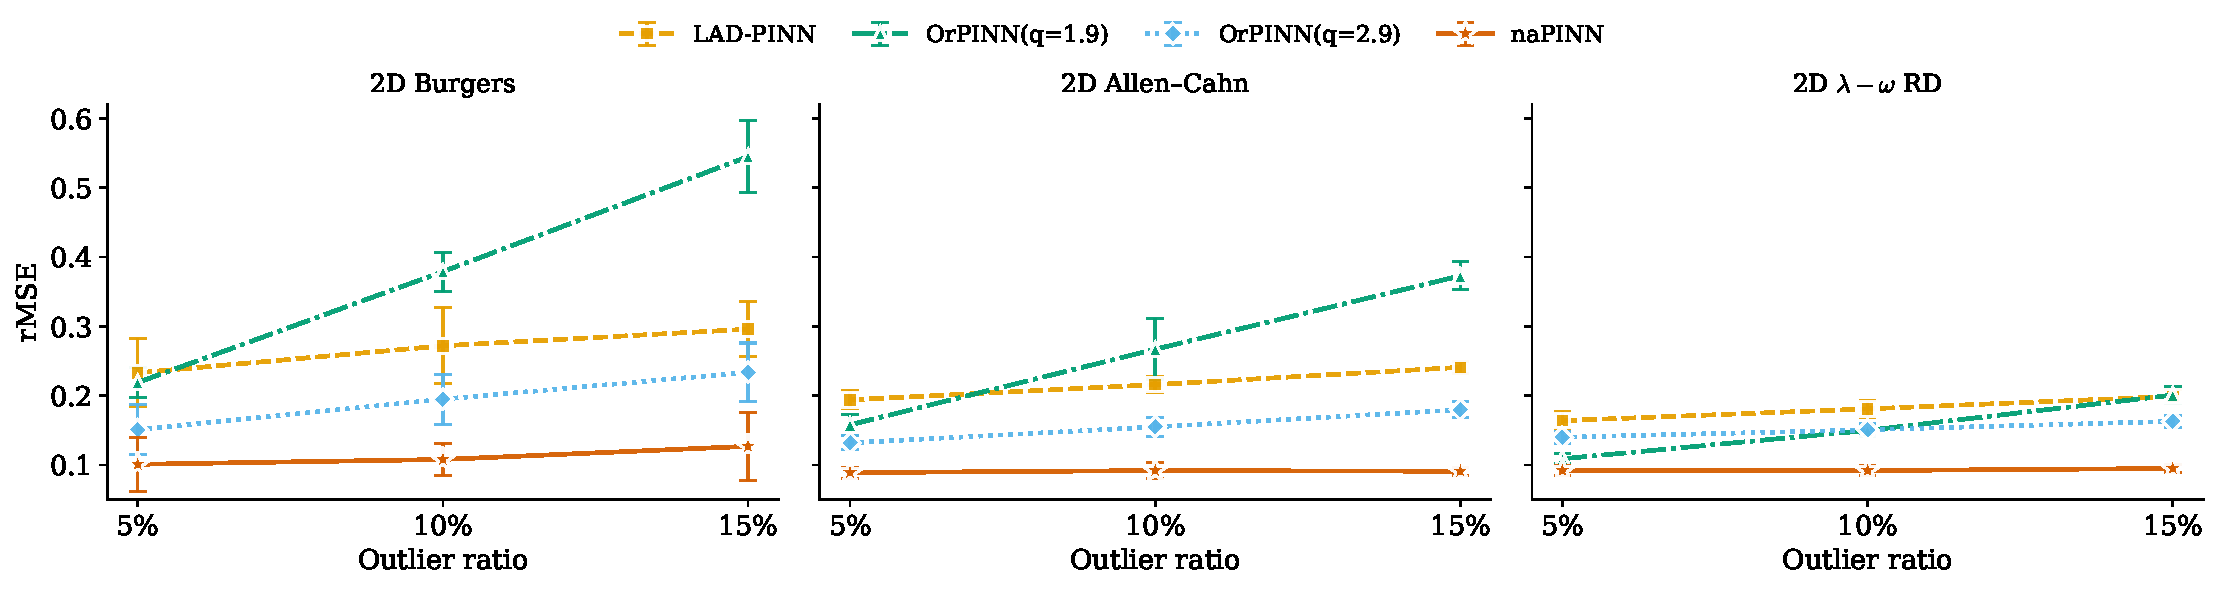
\includegraphics[width=\textwidth]{figures/ratio_curve.pdf}
\caption{Field rMSE against outlier ratio for the robust-loss baselines and
naPINN in the ten-trial experiments. Error bars are one standard deviation.}
\label{fig:ratio_curve}
\end{figure}



\paragraph{Coefficient recovery.}
Absolute error of the learned coefficient at $15\%$ outliers, mean (s.d.) over
seeds $40$--$42$ of the three-seed experiments, with relative error in brackets.
True values are $\varepsilon = 0.3$, $\nu = 0.01$ and $\beta = 1.0$.

\begin{center}\small
\setlength{\tabcolsep}{5pt}
\begin{tabular}{lccc}
\toprule
Method & $\varepsilon$ (Allen--Cahn) & $\nu$ (Burgers) & $\beta$ ($\lambda$--$\omega$) \\
\midrule
PINN (MSE)       & \pmstd{0.00355}{0.00163} [1.18\%] & \pmstd{0.00566}{0.00085} [56.6\%] & \pmstd{0.328}{0.005} [32.8\%] \\
LAD-PINN         & \pmstd{0.00312}{0.00088} [1.04\%] & \pmstd{0.00181}{0.00073} [18.1\%] & \pmstd{0.0837}{0.0041} [8.37\%] \\
OrPINN ($q = 1.9$) & \pmstd{0.00606}{0.00274} [2.02\%] & \pmstd{0.00515}{0.00080} [51.5\%] & \pmstd{0.0609}{0.0053} [6.09\%] \\
OrPINN ($q = 2.9$) & \pmstd{0.00321}{0.00060} [1.07\%] & \pmstd{0.00123}{0.00074} [12.3\%] & \pmstd{0.0523}{0.0040} [5.23\%] \\
PINN-EBM         & \pmstd{\textbf{0.00215}}{0.00036} [0.72\%] & \pmstd{\textbf{0.00065}}{0.00018} [6.46\%] & \pmstd{\textbf{0.0102}}{0.0041} [1.02\%] \\
naPINN           & \pmstd{\underline{0.00275}}{0.00048} [0.92\%] & \pmstd{\underline{0.00072}}{0.00021} [7.20\%] & \pmstd{\underline{0.0136}}{0.0007} [1.36\%] \\
\bottomrule
\end{tabular}
\end{center}

\noindent
Field reconstruction and coefficient identification are separate goals, and we
report them separately. naPINN and PINN-EBM recover all three coefficients with
similar accuracy, and the small Burgers viscosity is the hardest case for every
method.

\paragraph{Update-count control.}
Giving PINN (MSE) $35{,}000$ rather than $30{,}000$ updates (three-seed experiments)
leaves its rMAE at $0.875$/$0.592$/$0.448$ on
Allen--Cahn/Burgers/$\lambda$--$\omega$. The wall-clock-matched control is in
\cref{app:compute}.

\section{ADDITIONAL RESULTS ON REAL MEASUREMENTS}
\label{app:real}

\paragraph{Data.}
The Cylinder data have $200$ frames at $192$ fixed, irregularly placed training
sensors, which gives $38{,}400$ velocity vectors for training. Evaluation uses
$1{,}549{,}400$ held-out velocity vectors at $7{,}747$ locations disjoint from the
training sensors.

\paragraph{All methods on the Cylinder data.}
The table below gives the held-out errors of all eight methods on the Cylinder
data, mean (s.d.) over seeds $40$--$42$, with the best in bold and the second best
underlined. naPINN has the lowest error in every column, and its standard
deviation is at least five times smaller than that of PINN-EBM at either weight.

\begin{center}\small
\begin{tabular}{lcccc}
\toprule
 & \multicolumn{2}{c}{$10\%$} & \multicolumn{2}{c}{$15\%$} \\
\cmidrule(lr){2-3}\cmidrule(lr){4-5}
Method & rMAE & rMSE & rMAE & rMSE \\
\midrule
PINN (MSE) & \pmstd{0.406}{0.001} & \pmstd{0.429}{0.001} & \pmstd{0.574}{0.004} & \pmstd{0.591}{0.006} \\
LAD-PINN & \pmstd{0.246}{0.007} & \pmstd{0.278}{0.005} & \pmstd{0.270}{0.005} & \pmstd{0.300}{0.004} \\
OrPINN ($q = 2.9$) & \pmstd{0.214}{0.004} & \pmstd{\underline{0.250}}{0.004} & \pmstd{0.231}{0.005} & \pmstd{0.265}{0.004} \\
PINN-EBM ($\wpde = 1$) & \pmstd{0.370}{0.045} & \pmstd{0.425}{0.040} & \pmstd{0.424}{0.016} & \pmstd{0.464}{0.016} \\
PINN-EBM ($\wpde = 50$) & \pmstd{0.224}{0.019} & \pmstd{0.331}{0.018} & \pmstd{0.336}{0.111} & \pmstd{0.414}{0.073} \\
naPINN-L1 & \pmstd{0.220}{0.010} & \pmstd{0.262}{0.009} & \pmstd{0.226}{0.008} & \pmstd{0.270}{0.008} \\
naPINN-$q$2.9 & \pmstd{\underline{0.206}}{0.001} & \pmstd{0.252}{0.004} & \pmstd{\underline{0.216}}{0.006} & \pmstd{\underline{0.261}}{0.005} \\
\midrule
naPINN & \pmstd{\textbf{0.155}}{0.002} & \pmstd{\textbf{0.215}}{0.003} & \pmstd{\textbf{0.160}}{0.001} & \pmstd{\textbf{0.223}}{0.003} \\
\bottomrule
\end{tabular}
\end{center}

\paragraph{Combining naPINN with robust losses.}
At $15\%$ corrupted rows on the Cylinder data, naPINN-L1 reaches held-out
rMAE\,/\,rMSE of $0.226$\,/\,$0.270$ and naPINN-$q$2.9 reaches
$0.216$\,/\,$0.261$, against $0.160$\,/\,$0.223$ for naPINN with the squared
loss. Both combinations still have lower error than PINN-EBM
($0.336$\,/\,$0.414$ at $\wpde = 50$). On this corruption the squared loss is the
better choice inside the gate.

\paragraph{Additional scenarios.}
We also ran all eight methods on three other RealPDEBench scenarios (Controlled
Cylinder, FSI and Foil) at $10\%$ and $15\%$ corrupted rows with seeds
$40$--$42$, $144$ runs in total, with the design fixed before any run. naPINN has the lowest mean rMAE in all six
dataset--severity conditions and the lowest mean rMSE in four, while OrPINN with
$q = 2.9$ has the lowest rMSE on FSI at both severities. The table below gives
the held-out errors, mean (s.d.) over the three seeds, with the best in bold and
the second best underlined. On Foil at $15\%$, naPINN-$q$2.9 reaches an rMAE
of $1.68$ on one seed, which explains its large mean and spread. The RealPDEBench
Combustion scenario was excluded because its measurement is a single
chemiluminescence intensity channel, not a velocity field.

\begin{center}\small
\resizebox{\textwidth}{!}{%
\begin{tabular}{llcccccc}
\toprule
 & & \multicolumn{2}{c}{Controlled Cylinder} & \multicolumn{2}{c}{FSI} & \multicolumn{2}{c}{Foil} \\
\cmidrule(lr){3-4}\cmidrule(lr){5-6}\cmidrule(lr){7-8}
Method & Metric & $10\%$ & $15\%$ & $10\%$ & $15\%$ & $10\%$ & $15\%$ \\
\midrule
\multirow{2}{*}{PINN (MSE)}
 & rMAE & \pmstd{0.404}{0.003} & \pmstd{0.563}{0.008} & \pmstd{0.564}{0.011} & \pmstd{0.690}{0.003} & \pmstd{0.386}{0.004} & \pmstd{0.552}{0.012} \\
 & rMSE & \pmstd{0.415}{0.004} & \pmstd{0.564}{0.007} & \pmstd{0.680}{0.011} & \pmstd{0.774}{0.001} & \pmstd{0.398}{0.004} & \pmstd{0.560}{0.012} \\
\cmidrule(lr){2-8}
\multirow{2}{*}{LAD-PINN}
 & rMAE & \pmstd{0.247}{0.006} & \pmstd{0.271}{0.006} & \pmstd{0.451}{0.015} & \pmstd{0.466}{0.006} & \pmstd{0.224}{0.007} & \pmstd{0.246}{0.004} \\
 & rMSE & \pmstd{0.269}{0.005} & \pmstd{0.291}{0.005} & \pmstd{\underline{0.618}}{0.020} & \pmstd{\underline{0.625}}{0.002} & \pmstd{0.246}{0.006} & \pmstd{0.266}{0.004} \\
\cmidrule(lr){2-8}
\multirow{2}{*}{OrPINN ($q = 2.9$)}
 & rMAE & \pmstd{0.226}{0.006} & \pmstd{0.239}{0.006} & \pmstd{\underline{0.425}}{0.002} & \pmstd{\underline{0.436}}{0.002} & \pmstd{0.196}{0.008} & \pmstd{0.215}{0.010} \\
 & rMSE & \pmstd{0.252}{0.003} & \pmstd{0.263}{0.004} & \pmstd{\textbf{0.609}}{0.006} & \pmstd{\textbf{0.615}}{0.009} & \pmstd{0.222}{0.006} & \pmstd{0.239}{0.008} \\
\cmidrule(lr){2-8}
\multirow{2}{*}{PINN-EBM ($\wpde = 1$)}
 & rMAE & \pmstd{0.342}{0.169} & \pmstd{0.258}{0.130} & \pmstd{0.703}{0.032} & \pmstd{0.728}{0.019} & \pmstd{0.289}{0.053} & \pmstd{0.239}{0.106} \\
 & rMSE & \pmstd{0.426}{0.198} & \pmstd{0.309}{0.104} & \pmstd{0.764}{0.007} & \pmstd{0.771}{0.012} & \pmstd{0.306}{0.051} & \pmstd{0.262}{0.095} \\
\cmidrule(lr){2-8}
\multirow{2}{*}{PINN-EBM ($\wpde = 50$)}
 & rMAE & \pmstd{0.283}{0.024} & \pmstd{0.256}{0.118} & \pmstd{0.591}{0.133} & \pmstd{0.542}{0.063} & \pmstd{0.291}{0.133} & \pmstd{0.442}{0.394} \\
 & rMSE & \pmstd{0.365}{0.033} & \pmstd{0.304}{0.097} & \pmstd{0.773}{0.061} & \pmstd{0.757}{0.067} & \pmstd{0.310}{0.124} & \pmstd{0.468}{0.369} \\
\cmidrule(lr){2-8}
\multirow{2}{*}{naPINN-L1}
 & rMAE & \pmstd{\underline{0.217}}{0.002} & \pmstd{\underline{0.222}}{0.003} & \pmstd{0.464}{0.005} & \pmstd{0.466}{0.000} & \pmstd{0.188}{0.021} & \pmstd{\underline{0.210}}{0.025} \\
 & rMSE & \pmstd{\underline{0.243}}{0.002} & \pmstd{\underline{0.249}}{0.004} & \pmstd{0.664}{0.005} & \pmstd{0.681}{0.009} & \pmstd{0.215}{0.018} & \pmstd{\underline{0.234}}{0.022} \\
\cmidrule(lr){2-8}
\multirow{2}{*}{naPINN-$q$2.9}
 & rMAE & \pmstd{0.254}{0.059} & \pmstd{0.265}{0.055} & \pmstd{0.526}{0.063} & \pmstd{0.500}{0.029} & \pmstd{\underline{0.186}}{0.026} & \pmstd{0.700}{0.848} \\
 & rMSE & \pmstd{0.278}{0.053} & \pmstd{0.287}{0.051} & \pmstd{0.697}{0.059} & \pmstd{0.699}{0.022} & \pmstd{\underline{0.214}}{0.022} & \pmstd{0.718}{0.836} \\
\midrule
\multirow{2}{*}{naPINN}
 & rMAE & \pmstd{\textbf{0.149}}{0.003} & \pmstd{\textbf{0.152}}{0.007} & \pmstd{\textbf{0.399}}{0.001} & \pmstd{\textbf{0.418}}{0.002} & \pmstd{\textbf{0.100}}{0.004} & \pmstd{\textbf{0.118}}{0.024} \\
 & rMSE & \pmstd{\textbf{0.200}}{0.003} & \pmstd{\textbf{0.202}}{0.007} & \pmstd{0.646}{0.003} & \pmstd{0.680}{0.007} & \pmstd{\textbf{0.152}}{0.002} & \pmstd{\textbf{0.164}}{0.016} \\
\bottomrule
\end{tabular}%
}
\end{center}


\section{ABLATION DETAILS}
\label{app:ablations}

\paragraph{Gate classification.}
Trained gate on Allen--Cahn at $10\%$ outliers, with percentages of all
measurements.

\begin{center}\small
\begin{tabular}{lcc}
\toprule
True label & Excluded & Included \\
\midrule
Corrupted & $2{,}209$ ($9.8\%$) & $41$ ($0.2\%$) \\
Clean  & $152$ ($0.7\%$) & $20{,}098$ ($89.3\%$) \\
\bottomrule
\end{tabular}
\end{center}

\noindent
The few errors come from the overlap between the smallest outlier offsets and
the skewed tail of the background noise, where the two distributions overlap.

\paragraph{Frozen gate.}
Warm-up and the learned EBM are kept, and cutoff and steepness are held at their
initial values $\tilde\tau = 2$, $\tilde a = 30$ and $\rej = 0$. Because the gate weights
carry no gradient to $\theta$ and the gate parameters are frozen, the rejection
term is constant, so setting $\rej = 0$ changes nothing and the ablation differs
from naPINN only in whether the gate is trained.

\paragraph{Residual-magnitude gate.}
The gate $\sig(a(\tau - |\tilde r|))$ with trainable $a, \tau$ and the same
rejection cost $0.5$, initialized at $\tilde\tau = 1$, $\tilde a = 10$, with no density
estimator.
The fixed-quantile selector uses $\sig(10(q_{0.95} - |\tilde r|))$, where
$q_{0.95}$ is the minibatch $95\%$ quantile of $|\tilde r|$.

\paragraph{Pre-training screens.}
\label{app:screens}
Every training measurement is scored, a measurement row is flagged if the score
of any component exceeds a threshold $k$, flagged rows are removed, and an ordinary
PINN (MSE) is trained on the rest for $30{,}000$ updates. The scores are
$|y - \mathrm{mean}|/\mathrm{sd}$, $|y - \mathrm{median}|/(1.4826\,
\mathrm{MAD})$, and the MAD-standardized deviation of $y$ from $\tilde m$, the
median of the measurement's $16$ nearest neighbors in space and time. The threshold was chosen once on a separate calibration seed by
detection F1 against the true corruption labels and then frozen, and no field error
was inspected. The selected $k$ is $1.5$ in two, $2.0$ in five and $2.5$ in two
of the nine screen--benchmark cells, so no single value serves.

\paragraph{Screen removal diagnostics.}
The three columns are fractions of three different totals. Exactly $15.00\%$ of
rows are corrupted, and values are in Allen--Cahn\,/\,Burgers\,/\,$\lambda$--$\omega$
order.

\begin{center}\small
\begin{tabular}{lccc}
\toprule
 & \multicolumn{3}{c}{Rows removed, as a fraction of \dots} \\
\cmidrule(lr){2-4}
Screen & all rows & the corrupted $15\%$ & the clean $85\%$ \\
\midrule
Global $z$-score     & 13.4 / 17.9 / 9.6\% & 54.1 / 81.9 / 63.5\% & 6.24 / 6.59 / 0.02\% \\
Global MAD           & 13.3 / 14.8 / 12.8\% & 60.0 / 84.5 / 82.9\% & 5.04 / 2.44 / 0.35\% \\
Neighborhood median  & 14.5 / 14.8 / 14.8\% & 90.1 / 98.3 / 98.0\% & 1.11 / 0.02 / 0.04\% \\
\bottomrule
\end{tabular}
\end{center}

\noindent
For example, Allen--Cahn has $22{,}500$ measurement rows, $3{,}375$ corrupted.
The global $z$-score screen removes $3{,}020$ of them, namely $1{,}827$ corrupted
($54.1\%$ of $3{,}375$) and $1{,}193$ clean ($6.24\%$ of $19{,}125$).

\paragraph{Warm-up.}
Removing the warm-up at the original budget appeared to matter on Allen--Cahn
(rMAE $0.638$ without against $0.134$ with, five trials), but that comparison also
removes $5{,}000$ updates. At a matched budget, with the joint stage receiving all
$30{,}000$ updates, rMAE is $0.090$/$0.081$/$0.077$ without warm-up against
$0.092$/$0.082$/$0.071$ with it, so the warm-up does not change accuracy. We keep
it so that the estimator is first fitted to residuals of a
partly trained network.

\paragraph{Estimator.}
EBM, Gaussian mixture and kernel density estimate in the same pipeline,
ten-trial experiments. The choice does not change the conclusions. The mixture and
kernel estimates match or beat the EBM on Allen--Cahn at some ratios, while the
EBM is best or tied on Burgers and $\lambda$--$\omega$ at every ratio. We keep the EBM as
the default because it is a flexible trainable density that needs no choice of
component count or bandwidth.

\begin{center}\small
\setlength{\tabcolsep}{4pt}
\begin{tabular}{llcccccc}
\toprule
& & \multicolumn{2}{c}{$5\%$} & \multicolumn{2}{c}{$10\%$} & \multicolumn{2}{c}{$15\%$} \\
\cmidrule(lr){3-4}\cmidrule(lr){5-6}\cmidrule(lr){7-8}
Benchmark & Estimator & rMAE & rMSE & rMAE & rMSE & rMAE & rMSE \\
\midrule
\multirow{3}{*}{Allen--Cahn}
 & EBM & 0.104 & 0.101 & 0.110 & 0.108 & 0.134 & 0.127 \\
 & GMM & 0.110 & 0.110 & 0.081 & 0.082 & 0.117 & 0.113 \\
 & KDE & 0.132 & 0.121 & 0.117 & 0.110 & 0.090 & 0.091 \\
\midrule
\multirow{3}{*}{Burgers}
 & EBM & 0.075 & 0.089 & 0.074 & 0.092 & 0.072 & 0.091 \\
 & GMM & 0.083 & 0.101 & 0.085 & 0.103 & 0.093 & 0.106 \\
 & KDE & 0.086 & 0.096 & 0.104 & 0.109 & 0.101 & 0.109 \\
\midrule
\multirow{3}{*}{$\lambda$--$\omega$}
 & EBM & 0.073 & 0.092 & 0.074 & 0.092 & 0.076 & 0.095 \\
 & GMM & 0.078 & 0.092 & 0.081 & 0.096 & 0.082 & 0.096 \\
 & KDE & 0.083 & 0.100 & 0.090 & 0.105 & 0.083 & 0.100 \\
\bottomrule
\end{tabular}
\end{center}

\paragraph{Other noise families.}
On $\lambda$--$\omega$ at $15\%$ outliers with a Laplace or Gaussian background
(rMSE, ten trials), naPINN with the squared loss does not beat LAD-PINN or OrPINN, but the
same gate with an $\ell_1$ reconstruction loss does. The gate composes with an
appropriate reconstruction loss, but it does not replace the choice of one.

\begin{center}\small
\setlength{\tabcolsep}{8pt}
\begin{tabular}{lcc}
\toprule
Method & Laplace & Gaussian \\
\midrule
PINN (MSE) & 0.323 & 0.326 \\
LAD-PINN & 0.085 & 0.109 \\
OrPINN ($q = 2.9$) & 0.081 & 0.107 \\
naPINN & 0.085 & 0.126 \\
naPINN-L1 & \textbf{0.059} & \textbf{0.064} \\
naPINN-$q$2.9 & \underline{0.071} & \underline{0.067} \\
\bottomrule
\end{tabular}
\end{center}

\section{BACKBONE ARCHITECTURES}
\label{app:backbone}

The MLP backbone is replaced by FLS, whose input layer is a learnable sinusoidal
feature map \citep{Wong2022FLS}, QRes, which adds a multiplicative term
$(W_1 x)\odot(W_2 x)$ to each layer \citep{Bu2021QRes}, PirateNet, with random
Fourier embeddings and gated residual blocks \citep{Wang2024PirateNet}, and KAN,
with learnable B-spline activations \citep{Liu2024KAN}. Each is trained with the
vanilla objective and with naPINN, everything else fixed. Every backbone is
reproduced from its authors' reference code, takes the space--time coordinates as input, ends in a
linear head, and uses five layers (or blocks) of width $80$ unless stated otherwise.
\begin{itemize}
\item \emph{FLS.} The first layer is $\gamma(x) = \sin(2\pi(W_1x + b_1))$ with
trainable $W_1 \sim \mathcal{N}(0, 1)$ and $b_1 = 0$ at initialization,
followed by four $\tanh$ layers.
\item \emph{QRes.} Each layer computes $(W_1x)\odot(W_2x) + W_1x + b$
followed by $\tanh$, as in the reference implementation.
\item \emph{PirateNet.} A fixed Gaussian Fourier embedding
$\gamma(x) = [\cos Bx; \sin Bx]$ with scale $1.0$ and dimension $80$ feeds two
gating projections $U, V$. Each of five residual blocks mixes $U$ and $V$
through three $\tanh$ layers and adds a skip $x_{\ell+1} = \alpha_\ell h_\ell +
(1-\alpha_\ell)x_\ell$ with $\alpha_\ell$ trainable and initialized at zero.
\item \emph{KAN.} Each connection is $w^{\mathrm{base}}\,\mathrm{SiLU}(z) +
w^{\mathrm{spline}}\sum_k c_k B_k(z)$ with cubic B-splines on a grid of size
$5$. The first layer's grid covers the domain bounds, and later layers use
$[-1,1]$.
\end{itemize}
Parameter counts are $26{,}402$ (MLP, FLS), $52{,}242$ (QRes), $110{,}327$
(PirateNet) and $260{,}000$ (KAN) for two outputs. They are not matched,
because the question is whether the gain transfers across families. As
\cref{tab:backbone} shows, naPINN reduces the error of the plain PINN on every
backbone and benchmark, by a factor of $3.2$ to $7.7$. The best backbone varies by benchmark, so the main
experiments keep the MLP.

\begin{table}[h]
\centering
\small
\caption{Backbone ablation at $10\%$ outliers, ten trials. Best in bold, second
best underlined.}
\label{tab:backbone}
\vspace{4pt}
\setlength{\tabcolsep}{5pt}
\begin{tabular}{llcccccc}
\toprule
& & \multicolumn{2}{c}{Allen--Cahn} & \multicolumn{2}{c}{Burgers} & \multicolumn{2}{c}{$\lambda$--$\omega$} \\
\cmidrule(lr){3-4}\cmidrule(lr){5-6}\cmidrule(lr){7-8}
Backbone & Method & rMAE & rMSE & rMAE & rMSE & rMAE & rMSE \\
\midrule
\multirow{2}{*}{MLP}
 & Vanilla & 0.584 & 0.488 & 0.387 & 0.377 & 0.273 & 0.292 \\
 & naPINN  & 0.110 & 0.108 & \textbf{0.074} & 0.092 & 0.074 & 0.092 \\
\cmidrule(lr){1-8}
\multirow{2}{*}{KAN}
 & Vanilla & 0.564 & 0.473 & 0.397 & 0.393 & 0.269 & 0.293 \\
 & naPINN  & 0.110 & 0.105 & 0.085 & \underline{0.091} & \underline{0.055} & 0.069 \\
\cmidrule(lr){1-8}
\multirow{2}{*}{FLS}
 & Vanilla & 0.617 & 0.513 & 0.417 & 0.403 & 0.259 & 0.285 \\
 & naPINN  & \textbf{0.080} & \textbf{0.073} & \underline{0.080} & \textbf{0.088} & \underline{0.055} & \underline{0.068} \\
\cmidrule(lr){1-8}
\multirow{2}{*}{QRes}
 & Vanilla & 0.593 & 0.497 & 0.394 & 0.388 & 0.240 & 0.269 \\
 & naPINN  & \underline{0.103} & \underline{0.097} & 0.085 & 0.092 & 0.057 & 0.069 \\
\cmidrule(lr){1-8}
\multirow{2}{*}{PirateNet}
 & Vanilla & 0.615 & 0.522 & 0.400 & 0.396 & 0.253 & 0.278 \\
 & naPINN  & 0.113 & 0.108 & 0.079 & \textbf{0.088} & \textbf{0.046} & \textbf{0.056} \\
\bottomrule
\end{tabular}
\end{table}

\section{SENSITIVITY}
\label{app:sensitivity}

\paragraph{Running-scale weight.}
Allen--Cahn, $15\%$, seeds $40$--$42$.

\begin{center}\small
\begin{tabular}{ccll}
\toprule
$m$ & decay $1-m$ & rMAE & rMSE \\
\midrule
0.01 & 0.99 & $0.108 \pm 0.037$ & $0.109 \pm 0.032$ \\
0.05 & 0.95 & $0.092 \pm 0.004$ & $0.095 \pm 0.002$ \\
0.10 & 0.90 & $0.086 \pm 0.009$ & $0.092 \pm 0.005$ \\
\bottomrule
\end{tabular}
\end{center}

\noindent
$m = 0.01$ is the most seed-variable, and the differences lie within its seed
variation, so we claim insensitivity over this range but no optimal value.

\paragraph{Gate initialization.}
One factor at a time, Allen--Cahn, $15\%$, seeds $40$--$42$.

\begin{center}\small
\begin{tabular}{ll}
\toprule
Setting & rMAE mean $\pm$ s.d. \\
\midrule
$\tilde\tau = 2$, $\tilde a = 30$ (used) & $0.092 \pm 0.004$ \\
$\tilde\tau = 1$            & $0.100 \pm 0.027$ \\
$\tilde\tau = 4$            & $0.128 \pm 0.045$ \\
$\tilde a = 10$             & $0.083 \pm 0.019$ \\
$\tilde a = 60$             & $0.197 \pm 0.184$ \\
\bottomrule
\end{tabular}
\end{center}

\noindent
The sharpest initial gate ($\tilde a = 60$) has the worst mean and the largest spread
because one of its three seeds diverged, and $\tilde\tau = 4$ is also worse on average.
The other settings stay within the seed variation of the default. The default
values were not selected on performance.

\paragraph{Rejection cost.}
\Cref{fig:rej_cost} sweeps $\rej$ on Allen--Cahn at $15\%$. Accuracy is flat
between $0.1$ and $0.8$, worse without the term, and degrades sharply at $0.9$ and above,
where by \cref{prop:gate}(b) the price of exclusion exceeds the squared residuals
near the cutoff and the gate stops excluding corrupted measurements.

\begin{figure}[h]
\centering
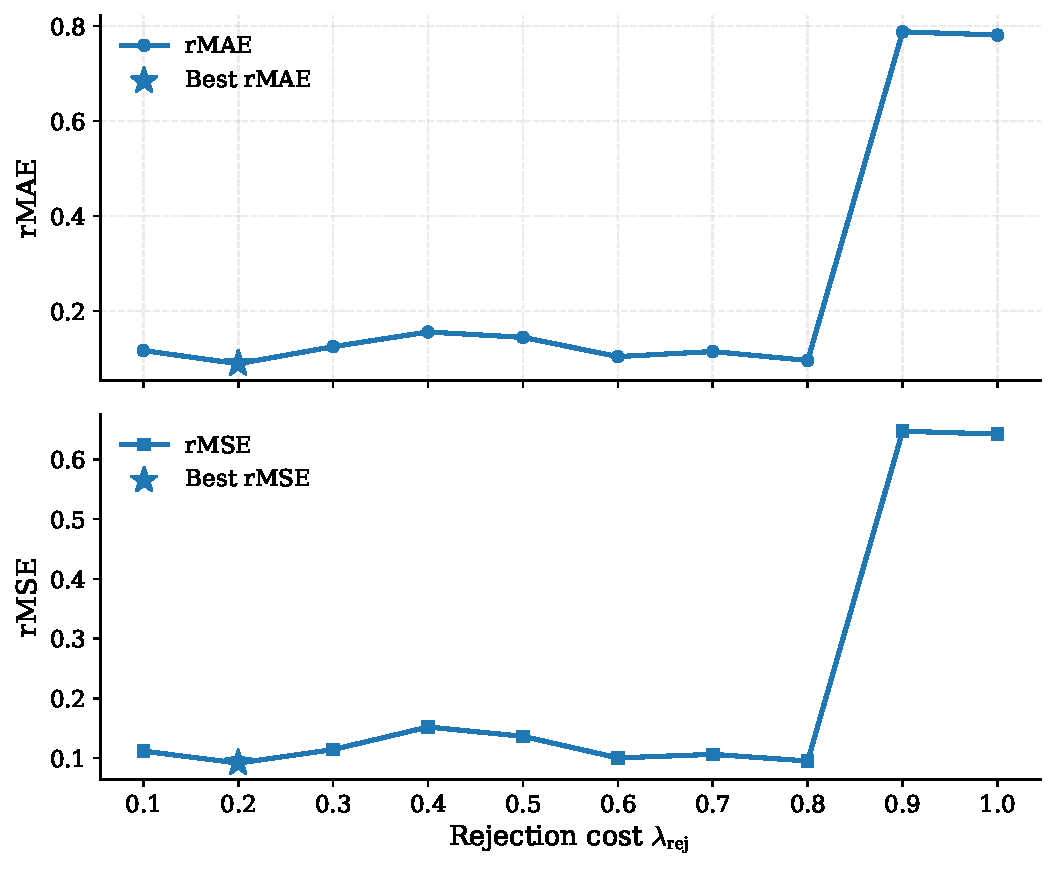
\includegraphics[width=0.55\linewidth]{figures/rej_cost.pdf}
\caption{Sensitivity to the rejection cost on Allen--Cahn at $15\%$ outliers, showing
rMAE (top) and rMSE (bottom) against $\rej$.}
\label{fig:rej_cost}
\end{figure}

\paragraph{Gate parameters during training.}
\Cref{fig:gate_params} tracks the pre-softplus cutoff $\tilde\tau$ and steepness
$\tilde a$ on $\lambda$--$\omega$. The cutoff settles within a few thousand joint updates, at
about $2.8$, $1.8$ and $1.3$ for $5\%$, $10\%$ and $15\%$ outliers. Under heavier
corruption the gate excludes measurements that are less far below the mean
log-density, consistent with \cref{prop:gate}(b). The steepness rises
throughout, so the gate sharpens from a soft weighting into a nearly hard
decision and treats the included measurements almost uniformly.

\begin{figure}[h]
\centering
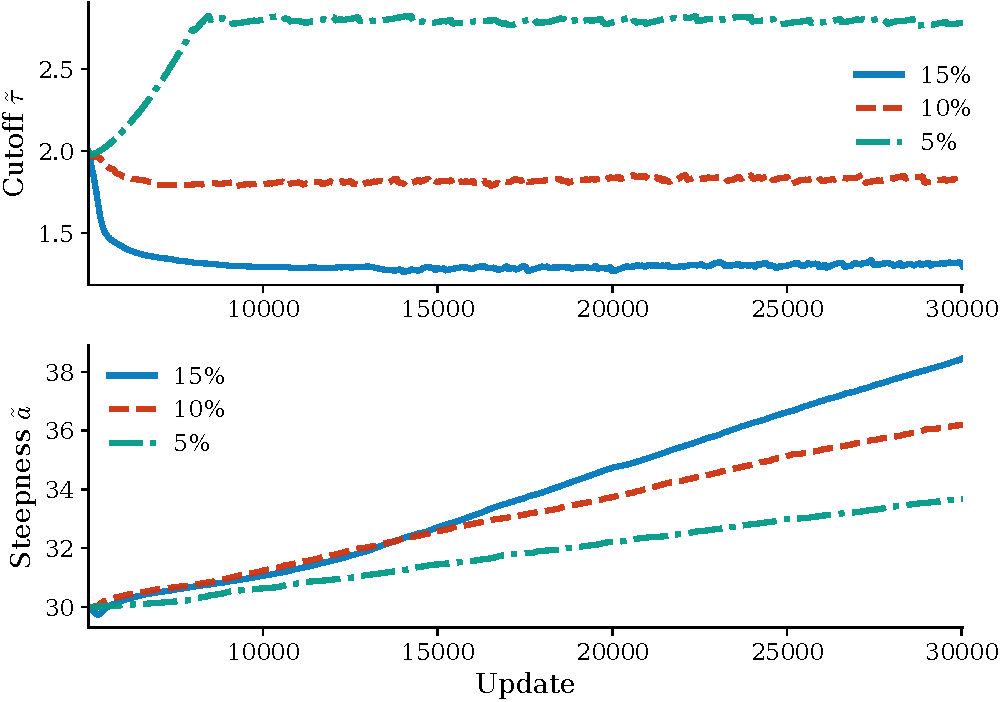
\includegraphics[width=0.55\linewidth]{figures/gate_params.pdf}
\caption{Pre-softplus cutoff $\tilde\tau$ (top) and steepness $\tilde a$ (bottom) during joint training on
$\lambda$--$\omega$ at three outlier ratios.}
\label{fig:gate_params}
\end{figure}

\section{COMPUTE}
\label{app:compute}

The $30{,}000$-update budget counts PINN parameter updates. Seconds per update on
one NVIDIA RTX A6000 at $15\%$ corruption with the EBM estimator are listed below.

\begin{center}\small
\setlength{\tabcolsep}{8pt}
\begin{tabular}{lcc}
\toprule
Benchmark & PINN & naPINN \\
\midrule
Allen--Cahn & 0.0356 & 0.0397 \\
Burgers & 0.0423 & 0.0478 \\
$\lambda$--$\omega$ & 0.0458 & 0.0472 \\
\bottomrule
\end{tabular}
\end{center}

\noindent
The estimator initialization takes $46$--$49$\,s. Extrapolating these rates
over the budget gives $1{,}068$/$1{,}269$/$1{,}374$\,s for a standard PINN and
$1{,}239$/$1{,}482$/$1{,}464$\,s for naPINN, with initialization $3$--$4\%$ of the
naPINN total. This slightly overestimates naPINN, since it charges the joint
rate to the warm-up.

\paragraph{Equal elapsed time.}
On a reserved GPU each fixed-loss baseline received exactly naPINN's measured
end-to-end time ($1{,}265$/$1{,}201$/$1{,}308$\,s), which allowed on average
$37{,}561$ to $53{,}494$ PINN updates, depending on the baseline and benchmark.
The mean number of updates over seeds $40$--$42$ is given below.

\begin{center}\small
\setlength{\tabcolsep}{8pt}
\begin{tabular}{lccc}
\toprule
Benchmark & OrPINN ($q = 2.9$) & LAD-PINN & PINN (MSE) \\
\midrule
Allen--Cahn & $48{,}562$ & $47{,}296$ & $53{,}494$ \\
Burgers & $37{,}561$ & $40{,}311$ & $39{,}627$ \\
$\lambda$--$\omega$ & $39{,}167$ & $42{,}388$ & $39{,}186$ \\
\bottomrule
\end{tabular}
\end{center}

\noindent These times were measured in the control run itself and differ
from the extrapolation above, which combines per-update rates from a separate
timing run, and the control uses the measured times. Mean rMAE over seeds $40$--$42$ at $15\%$ is given below.

\begin{center}\small
\setlength{\tabcolsep}{8pt}
\begin{tabular}{lcccc}
\toprule
Benchmark & naPINN & OrPINN ($q = 2.9$) & LAD-PINN & PINN (MSE) \\
\midrule
Allen--Cahn & \textbf{0.092} & \underline{0.285} & 0.357 & 0.860 \\
Burgers & \textbf{0.082} & \underline{0.190} & 0.244 & 0.577 \\
$\lambda$--$\omega$ & \textbf{0.071} & \underline{0.137} & 0.198 & 0.427 \\
\bottomrule
\end{tabular}
\end{center}

\section{REPRODUCIBILITY}
\label{app:repro}

\paragraph{Experiment sets.}
The ten-trial experiments, with ten independent runs per setting, cover all
outlier ratios and every baseline in \cref{tab:exact}, together with the
backbone, estimator, normalization and noise-family ablations. The three-seed
experiments (seeds $40$--$42$, $15\%$ outliers) produced the ablation study, the
pre-training screens, the compute controls, the running-scale and
gate-initialization sweeps and the coefficient errors. The warm-up ablation at
the original budget uses five trials.

\paragraph{Settings.}
Every naPINN run uses running-scale weight $m = 0.05$, gate initialization
$\tilde\tau = 2$, $\tilde a = 30$ and rejection cost $\rej = 0.5$, and the sensitivity studies in
\cref{app:sensitivity} are the only exceptions. The screen thresholds were
selected on a separate calibration seed, and no naPINN setting was selected on a
reported seed.
The corruption generator is used at an intensity fixed before any run and leaves
held-out measurements unchanged. Burgers and $\lambda$--$\omega$ references are
generated numerically and Allen--Cahn is analytical. RealPDEBench (Cylinder,
Controlled Cylinder, FSI and Foil, release 2.0.0) is distributed under
CC BY-NC 4.0 \citep{hu2026realpdebench}.

\section{BROADER IMPACTS}
\label{app:impact}

More reliable recovery from imperfect measurements can help scientific and
engineering inference where repeating an experiment is costly. The same gate can
reject rare but valid behavior, or absorb model discrepancy into what looks like
a sensor-reliability decision, and its weights are not calibrated diagnoses of
sensor failure. In consequential uses, raw measurements should be retained, gate
decisions audited against domain knowledge, and conclusions checked against
independent measurements.

\end{document}
